\documentclass[]{article}
\usepackage{amsmath}
\usepackage{hyperref}
\usepackage{gensymb}
\usepackage{graphicx}
\usepackage{svg}
\usepackage{bbding}
\usepackage{mathtools}
\usepackage{centernot}
\usepackage{multicol}
\usepackage{lmodern}
\usepackage[left=10mm, top=10mm, right=10mm, bottom=10mm, nohead, nofoot]{geometry} %Exam
%\usepackage{bigints}

\DeclareFontFamily{OMX}{lmex}{}
\DeclareFontShape{OMX}{lmex}{m}{n}{<-> lmex10}{}

%\usepackage{babel}[english]
%opening
\title{114074 - Physics 1P}
\author{Noam Soker}
%	0545925995}

\parindent=0em
\setsvg{inkscape={"C:/Program Files/Inkscape/inkscape.exe" -z -C}}
%C:\Program Files\ImageMagick-7.0.3-Q16-HDRI
\begin{document}


\maketitle

\begin{abstract}

\end{abstract}
\section{Intro}

What is mass? Mass is kind of energy.


Course goals:
\begin{enumerate}
	\item Pleasure of lecturer 
	\item Recognize definitions in mechanics
	\item Recognize physical ideas
\end{enumerate}
 Energy is a conserved value as a result of time symmetry.
 
 
 \section{Mechanics}
 
 Movement of bodies
 
Galileo Galilei (1564-1642)

Nicolaus Copernicus (1473-1543)

Isaac Newton (1642-1727)

$\:$ Johannes Kepler

$\:$ Tycho Brahe

Albert Einstein
\subsection{vectors}
Vector is variable with value and direction.
\begin{itemize}
	\item  $\vec{A}$ - vector A
	\item  $\mid \vec{A} \mid$ or $A$ -  value of vector
	\item  $\hat{A}$  - unit vector in direction of $A$
\end{itemize}
\paragraph{Vector sum}
Both of vectors must be same unit.
$\vec{A}+\vec{B}$

\begin{center}
	\includegraphics[width=0.3\linewidth]{./lect1/pic1.png}
\end{center}

$\vec{A}+\vec{B}=\vec{A}+\vec{B}$ - Commutativity

\paragraph{Vector subtraction}

$$\vec{A}-\vec{B}=\vec{A}+(-\vec{B})$$

$-\vec{B}$ - opposite direction

$$\vec{A}+\vec{B}=-(\vec{A}+\vec{B})$$
\paragraph{Vector sum of multiple vectors} Order isn't important!
$\vec{A}+(\vec{B}+\vec{C})=(\vec{A}+\vec{B})+\vec{C}$ - Associativity

\begin{center}
	\includegraphics[width=0.3\linewidth]{./lect1/pic2.png}
\end{center}
\paragraph{Multiplication by scalar}
$k \cdot (\vec{A}+\vec{B})=k\cdot\vec{A}+k\cdot\vec{B}$ - Distributive

A physical quantity must fulfill following conditions to be a vector: 
\begin{enumerate}
	\item To have value and direction independent on coordination system
	\item Satisfy parallelogram law of vector sum (Commutativity)
\end{enumerate}
%$\vec{F}=(12N) \cdot (-\hat{y})$

\paragraph{Counter example to 2:}
Define turn of $90\degree$ around an axis according to right hand.
Turn around x and then y is not equal to turn y and then x. 
$\vec{A}+\vec{B}\neq\vec{A}+\vec{B}$
\paragraph{Vector multiplication} Don't have to be same unit.
\begin{enumerate}
	\item Scalar multiplication (dot product, inner product) - result is scalar. For $\vec{A}, \vec{B}$ with $\angle\vec{A}\vec{B}=\theta$ then $\vec{A}\cdot\vec{B}=\vec{B}\cdot\vec{A}=AB\cos\theta$.
	Product of vector A on projection of vector B on it.

\begin{center}	
	\includesvg[eps,svgpath = lect1/,width=0.2\linewidth]{pic3}
\end{center}
	
	For perpendicular vectors scalar product is $0$.
	
		Using components (Cartesian coordinate system):
		Define unit vector and axis($x,y,z$). Take vector $\vec{A}$ with angle $\theta$ to $x$.
		Take projection of $\vec{A}$ on axis: $A_x,A_y,A_z$. Then $\vec{A}=A_x\hat{x}+A_y\hat{y}+A_z\hat{z}$.
		
		$$\vec{A}\cdot\hat{x}=(A_x\hat{x}+A_y\hat{y}+A_z\hat{z})\cdot\hat{x}=A_x\hat{x}\cdot\hat{x}+A_y\hat{y}\cdot\hat{x}+A_z\hat{z}\cdot\hat{x}=A_x + 0 + 0 = A_x$$
		$$A=\sqrt{\vec{A}\cdot\vec{A}}=((A_x\hat{x}+A_y\hat{y}+A_z\hat{z})\cdot(A_x\hat{x}+A_y\hat{y}+A_z\hat{z}))^\frac{1}{2}=\sqrt{A_x^2 + A_y^2 + A_z^2}$$
		$$\hat{A}=\frac{\vec{A}}{\mid \vec{A} \mid}=\frac{A_x}{\mid \vec{A} \mid}\cdot\hat{x}$$
		$$\vec{A} \cdot \vec{B} = A_xB_x + A_yB_y$$
		$$\hat{A} \cdot \hat{B} = \frac{\vec{A}}{A} \cdot \frac{\vec{B}}{B} = \frac{\vec{A} \cdot \vec{B}}{A\cdot B} = \frac{AB\cos \alpha}{AB} = \cos \alpha$$
	\item Vector product (cross product) - $\vec{A} \times \vec{B}$
	
	$$\vec{C} = \vec{A} \times \vec{B} = -\vec{B} \times \vec{A}$$
	$$\vec{C} = \hat{c}AB\sin\alpha$$
	
	\subparagraph{Right hand rule:}
	
	Four fingers in direction of shortest path between $\vec{A}$ and $\vec{B}$, then thumb shows direction of $\vec{C}$.

\begin{center}	
	\includesvg[eps,svgpath = lect1/,width=0.2\linewidth]{pic4}
\end{center}
	
	$$\vec{A} \times \vec{A} = 0$$	
	$$\vec{A} \times(\vec{B} + \vec{C}) =  \vec{A} \times\vec{B} + \vec{A} \times\vec{C}$$
	
\end{enumerate}
\paragraph{Law of cosine}
\begin{center}	
	\includesvg[eps,svgpath = lect2/,width=0.2\linewidth]{pic1}
\end{center}
$$\vec{C} = \vec{A} - \vec{B}=\vec{A} + (-\vec{B})$$
$$(\vec{A}-\vec{B}) \cdot (\vec{A}-\vec{B}) = \vec{C} \cdot \vec{C}$$
$$A^2+B^2-2AB\cos \alpha = C^2$$

\paragraph{Power} Rate of doing work

$$W = LF\cos \alpha = \vec{L} \cdot \vec{F}$$

In a short time $dt$ a body passed a short distance $dL$.
So $dW=d\vec{L} \cdot {F}$

Then $power = \frac{dW}{dt} = \frac{d\vec{L}}{dt} \cdot \vec{F} = \vec{v} \cdot \vec{F}$


\subparagraph{Units} Units are:


Force  - $N$

Energy - $J$

Power -  $W$

\subsection{Cartesian coordinate system}

\begin{center}
	\includegraphics[width=0.2\linewidth]{./lect2/pic2.png}
\end{center}

\begin{align*}
\vec{A} \times \vec{B}  &\mathrlap{= (A_x\hat{x} + A_y\hat{y} + A_z\hat{z})\times (B_x\hat{x} + B_y\hat{y} + B_z\hat{z}) =}\\
&= A_xB_x(\hat{x} \times \hat{x}) &+ A_xB_y(\hat{x} \times \hat{y}) &+ A_xB_z(\hat{x} \times\hat{z})+\\ 
&&+A_yB_x(\hat{y} \times \hat{x}) &+ A_yB_y(\hat{y} \times \hat{y}) + A_yB_z(\hat{y} \times \hat{z}) +\\
&&&+ A_zB_x(\hat{z} \times \hat{x}) + A_zB_y(\hat{z} \times \hat{y}) + A_zB_z(\hat{z} \times \hat{z}) =\\
&&& = (A_yB_z -  A_zB_y)\hat{x}  + (A_zB_x + A_xB_z)\hat{y} + (A_xB_y - A_yB_x)\hat{z}
\end{align*}



\subsection{Usages}

\paragraph{Area of parallelogram}
\begin{center}	
	\includesvg[eps,svgpath = lect2/,width=0.5\linewidth]{pic3}
\end{center}
$h$ is an altitude.

$S  = ah = ab \sin \theta = \mid \vec{a} \times \vec{b} \mid\\
\vec{S} = \vec{a} \times \vec{b}$

If there is a curved surface area vector is perpendicular to surface in every point.
\paragraph{Parallelepiped volume}
\begin{center}	
	\includesvg[eps,svgpath = lect2/,width=0.7\linewidth]{pic4}
\end{center}
Two equal parallel parallelogram defined with $\vec{b}, \vec{c}$ and $\vec{a}$ is a vector between them.

$\vec{S} = \vec{b} \times \vec{c}\\
h = \mid \vec{a} \mid \cos \alpha\\
V = S \cdot h = \mid \vec{S} \cdot \vec{a} \mid = \mid (\vec{b} \times \vec{c}) \cdot \vec{a} \mid$

Same order (a,b,c), no matter which are used for cross product gives same result: $(\vec{a}\times \vec{b}) \cdot \vec{c} = \vec {b} \cdot (\vec{c} \times \vec{a})$. However different order (b,a,c), e.g. $(\vec{a}\times \vec{c}) \cdot \vec{b}$ will give opposite sign.

\paragraph{Law of sines}

$\vec{C} = \vec{A} + \vec{B}\\
\vec{A} \times \vec{C} = \vec{A} \times \vec{A}+ \vec{A} \times \vec{B} = \vec{A} \times \vec{B}\\
\mid \vec{A} \times \vec{C} \mid = \mid \vec{A} \times \vec{B}\mid\\
AC\sin \beta = AB\sin \gamma\\
\frac{C}{\sin \gamma} = \frac{B}{\sin \beta}$


\paragraph{Rate of covering of area}A stick of length L moves with velocity $\vec{v}$. $\vec{l}$ is perpendicular to stick and $| \vec{l} | = l$ and $\angle\vec{l}\vec{v}=\theta$


\begin{center}
	\includegraphics[width=0.4\linewidth]{./lect3/pic1.png}
\end{center}

What is area covered by a stick in time $\Delta t$?

$$dA = hl = \Delta tv \cos \theta l $$
$$\Delta t \rightarrow dt $$
$$\frac{dA}{dt} = vl \cos \theta = \vec{v} \cdot \vec{l}$$

\paragraph{Rate of covering of volume} Surface of area $\vec{S} = \vec{a} \times \vec{b}$.

\begin{center}
	\includegraphics[width=0.3\linewidth]{./lect3/pic2.png}
\end{center}

Volume is 
$$dV = (vdt) S \cos \theta $$
$$\frac{dV}{dt} = vS \cos \theta = \vec{v} \cdot \vec{S}$$


What is mass of air covered by surface per time?
$$\frac{d m_{air}}{dt}= V \cdot \rho_{air} = \vec{S} \cdot \vec{v} \rho_{air} $$
$$\frac{d m_{air}}{dt} = \dot{m}_{air} = \vec{S} \cdot \vec{v} \rho_{air} = \vec{S} \cdot \vec{\Phi_{air}}$$

$\vec{\Phi_{air}}= \left[\frac{kg}{m^2 sec}\right] =$ flux of mass of air.


\paragraph{Torque(moment of force)}


\begin{center}
	\includegraphics[width=0.3\linewidth]{./lect3/pic3.png}
\end{center}

$\vec{N} = \vec{r} \times \vec{F} \\
\vec{F} = \left[\frac{kg m}{s^2}\right] \\
\vec{r} = \left[m\right]\\
\vec{N} \left[\frac{kg \cdot m^2}{s^2}\right]$

$$\vec{N} = \vec{r} \times \vec{F} =  \vec{r}_1 \times \vec{F} = \vec{r}_{\perp} \times \vec{F} $$

\section{Derivatives of vector}

Derivative of position of body by time is velocity

$$\vec{v} = \frac{d\vec{r}}{dt} = \lim_{\Delta t \to 0} \frac{\Delta\vec{r}}{\Delta t}$$


\begin{center}
	\includegraphics[width=\linewidth]{./lect3/pic4.png}
\end{center}

$$\Delta \vec{r} = \vec{r}(t_2) - \vec{r}(t_1) $$
$$\vec{v} = \frac{d \vec{r}}{dt} = \frac{dx}{dt}\hat{x} + \frac{dy}{dt}\hat{y} + \frac{dz}{dt}\hat{z} $$
$v = | \vec{v} | = \sqrt{v_x^2 + v_y^2 + v_z^2}$ where $v_x = \frac{dx}{dt}$

\textbf{When coordinate system doesn't change with time}

\subsection{Coordinate system changing in time}

\begin{center}
	\includegraphics[width=0.25\linewidth]{./lect3/pic5.png}
\end{center}

$$\vec{r} = r \cdot \hat{r} $$
\begin{align*}
\left(\mbox{\FiveStarOpen}\right) &\vec{v} = \frac{d\vec{r}}{dt}= \frac{d}{dt} (r\hat{r}) = \frac{dr}{dt}\hat{r} + r \frac{d\hat{r}}{dt}
\end{align*}

\paragraph{Circle movement}

\begin{center}
	\includegraphics[width=0.4\linewidth]{./lect3/pic6.png}
\end{center}

Lets find $\Delta \hat{r}$ and $\Delta \hat{\theta}$. Move parallel beginnings of $\Delta \hat{r}$ to beginning of $\hat{r}$:

\begin{center}
	\includegraphics[width=0.4\linewidth]{./lect3/pic7.png}
\end{center}
$$\sin \alpha \simeq \alpha$$

$$\Delta \hat{r}  \parallel \hat{\theta} \perp \hat{r} $$
$$| \Delta \hat{r} | = | \hat{r} | \sin{\Delta \theta} = 1 \cdot \Delta \theta$$


Let's show that change in $\hat{r}$ is perpendicular to $\hat{r}$:

$$\frac{d}{dt}(1) = 0 = \frac{d}{dt}(\hat{r}\cdot\hat{r}) = \frac{d\hat{r}}{dt} \cdot \hat{r}+ \hat{r} \cdot \frac{d\hat{r}}{dt}$$
$$\hat{r} \cdot \frac{d\hat{r}}{dt} = 0$$
$$\hat{r} \perp \frac{d\hat{r}}{dt}$$

So $\Delta \hat{r} = (\Delta \theta) \cdot \hat{\theta}$
$$\frac{\Delta \hat{r}}{\Delta t} = \frac{(\Delta \theta) \cdot \hat{\theta}}{\Delta t}$$

When $\Delta t \to 0$

$$\frac{d \hat{r}}{d t} = \frac{(d \theta) \cdot \hat{\theta}}{d t}$$

Denote:

$$\omega = \frac{d \theta}{dt} $$

\begin{align*}
\left(\star\right) & \dot{\hat{r}} = \frac{d\hat{r}}{dt} = \omega \hat{\theta}
\end{align*}

\paragraph{$\Delta \hat{\theta}$} Similarly, direction of $\Delta \hat{\theta}$ is $-\hat{r}$ and $| \Delta \hat{\theta} | = \Delta\theta$

\begin{align*}
(\star\star) & \dot{\hat{\theta}} = \frac{d \hat{\theta}}{d t} = - \frac{d \theta}{dt} \hat{r}  = - \omega \hat{r}
\end{align*}
\begin{center}
	\includegraphics[scale=0.2]{./lect4/pic1.png}
\end{center}
\begin{align*}\left(\mbox{\FiveStarOpen\FiveStarOpen}\right) & \dot{\vec{r}} = \frac{dr}{dt} \cdot \hat{r} + r\frac{d\hat{r}}{dt} =  \frac{dr}{dt} \cdot \hat{r} + r \frac{(d \theta)}{d t}\cdot \hat{\theta}\end{align*}


\paragraph{Acceleration} $$\vec{a} = \frac{d\vec{v}}{dt} = \frac{d}{dt}\left( \frac{d\vec{r}}{dt} \right) = \frac{d^2\vec{r}}{dt^2}$$

Cartesian:

$$\vec{a} = \frac{d^2x}{dt^2}\hat{x} + \frac{d^2y}{dt^2}\hat{y} + \frac{d^2z}{dt^2}\hat{z}$$

Polar:

\begin{align*}\vec{a} = \frac{d\vec{v}}{dt} \stackrel{\mbox{\FiveStarOpen\FiveStarOpen}}{=} \frac{d}{dt}\left( \frac{dr}{dt}\hat{r} + r\frac{d\theta}{dt}\hat{\theta} \right) = \frac{d^2r}{dt^2}\hat{r} + \frac{dr}{dt} \cdot \frac{d\hat{r}}{dt} + \frac{dr}{dt}\cdot\frac{d\theta}{dt}\hat{\theta}  + r\frac{d^2\theta}{dt^2}\hat{\theta}  + r\frac{d\theta}{dt}\frac{d\hat{\theta}}{dt} =\\=
\frac{d^2r}{dt^2}\hat{r} + \frac{dr}{dt} \cdot \frac{d \theta }{d t} \cdot \hat{\theta}+ \frac{dr}{dt}\cdot\frac{d\theta}{dt}\hat{\theta}  + r\frac{d^2\theta}{dt^2}\hat{\theta}  - r\frac{d\theta}{dt}^2 \hat{r} = \left[ \frac{d^2 r}{dt^2} - r \frac{d\theta}{dt}^2\right]\hat{r} + \left[ 2 \frac{dr}{dt}\frac{d\theta}{dt} + r\frac{d^2\theta}{dt^2} \right]\hat{\theta}\end{align*}

$$\vec{a} = \left[ \frac{d^2r}{dt^2} - r\left( \frac{d\theta}{dt} \right)^2 \right]\hat{r} + \frac{1}{r} \left[ \frac{d}{dt}\left( r^2 \frac{d\theta}{dt} \right) \right]\hat{\theta}$$


\subsection{Check common cases}
\begin{enumerate}
	\item $\frac{{d\theta}}{dt} = 0 $
	
	$$	\vec{a} = \left[ \frac{d^2r}{dt^2} - 0 \right]\hat{r} + \frac{1}{r} \left[ \frac{d}{dt}\left( 0 \right) \right]\hat{\theta} =  \frac{d^2\vec{r}}{dt^2}$$
	\item $r = const $ and $\frac{d\theta}{dt} = \omega$
	
	$$\vec{a} = \left[ 0 - r\left( \frac{d\theta}{dt} \right)^2 \right]\hat{r} + \frac{1}{r} \left[ 0 \right]\hat{\theta} = -r\omega^2\hat{r}$$
\end{enumerate}

\paragraph{Circle motion} $r = const$ and $\frac{d\theta}{dt} = \omega = const$

\begin{center}
	\includegraphics[width=\linewidth]{./lect4/pic2.png}
\end{center}

$$\vec{v} = r \frac{d\theta}{dt}\hat{\theta} = r\omega\hat{\theta}$$

Let at $t=0$ $\theta=0$. At different time $t$ exist following connections:

$$\theta = \omega t$$

In Cartesian:

$$\vec{r} = x(t) \hat{x} + y(t) \hat{t} = r\cos\theta \hat{x} + r\sin\theta\hat{y}$$

Then:

$$\vec{r} = r \cos\left( \omega t\right) \hat{x} + r \sin \left( \omega t \right) \hat{y} $$

$$\vec{v} = \underbrace{- \omega r \sin \left( \omega t \right)}_{v_x} \hat{x} + \underbrace{\omega r \cos \left( \omega t \right)}_{v_y} \hat{y} $$

$$ v = \sqrt{v_x^2 + v_y^2} = \omega r $$

$$\vec{a} = - \omega^2r \cos \left( \omega t \right) \hat{x}  - \omega^2 r \sin \left( \omega t \right) \hat{y} = \omega^2 r \left[ \cos \left( \omega t \right) \hat{x} + \sin \left( \omega t \right) \hat{y} \right] = \omega^2 r \hat{r}$$


\section{Newton laws}
Isaak Newton(1643-1727)
\subsection{First law of Newton}
A body at rest or moving with constant velocity will keep its velocity unless there is force acting on body
\subsection{Second law of Newton}
The rate of change of momentum of a body, is directly proportional to the force applied.

$$\vec{F} = \frac{d\vec{p}}{dt} = \frac{d}{dt}\left(m\vec{v}\right) = \frac{dm}{dt}\vec{v} + m\frac{d\vec{v}}{dt}$$ 

If mass is constant:

$$\vec{F} = m\vec{a}$$

$m$ is inertial mass or mass.
\subsection{Third law of Newton}
When 2 bodies interact, the force first body exerts  on the second is equal in magnitude and opposite in direction to force second body exerts on the first.
\paragraph{Notes}
\begin{enumerate}
	\item Two forces are exerted on different bodies
	\item This law is connected to conservation of momentum
	\item Wrong in special relativity
\end{enumerate}

\paragraph{Example}

$$m\vec{a} = m\frac{d\vec{v}}{dt} = m \frac{d^2r}{dt^2} = m \ddot{\vec{r}}$$

If force is zero:

$$m\frac{d\vec{v}}{dt} = 0 $$

$$\vec{v} = \vec{v}_0 =const $$

$$\frac{d\vec{r}}{dt} = \vec{v}_0 $$

$$d\vec{r} = \vec{v}_0 dt$$

Find integral:

$$\int_{\vec{r}_{beg}}^{\vec{r}_{end}} d\vec{r} = \int_{t_{end}}^{t_{beg}} \vec{v} dt$$

$$\bigg[ \vec{r} \bigg]_{\vec{r}_0}^{\vec{r}} = \bigg[ \vec{v}_0 t \bigg]_{\vec{t}_0}^{\vec{t}}$$

$$\vec{r} - \vec{r}_0 = \vec{v}_t - \vec{v}_0t$$

$$\vec{r}(t) = \vec{r}_0 + \vec{v}_0\left( t-t_0 \right)$$

\subsection{Movement}
Movement is an equation describing position of body changing with a time
\paragraph{Second law} $$\vec{F} = m \vec{a} = m \ddot{\vec{r}} = m \frac{d^2 \vec{r}}{d t^2}$$ It's differential equation.

\paragraph{Example} Constant acceleration on surface Earth.

$$\vec{F} = - mg \hat{y}$$

Using second law for a constant mass:

$$\underbrace{m}_{\parbox{2cm}{\scriptsize  \centering gravitational\\ mass}} \frac{d^2 \vec{r}}{dt^2} = -\underbrace{m}_{\parbox{1cm}{\scriptsize  \centering inertial\\ mass}}g \hat{y}$$

$$-g\hat{y} = \hat{x} \frac{d^2x}{dt^2} + \hat{y}\frac{d^2y}{dt^2}$$

$$\frac{dx^2}{dt^2} = 0$$

$$\frac{d^2y}{dt^2}=-g$$

Solution is:

$$x_0 = x_0 + v_{x0}t$$

$$y= y_0 + v_{y0}t +- \frac{1}{2}gt^2$$

$$v_y = v_{y0} -gt$$
\paragraph{Gravitational field} $-g\hat{y}$

Examples:

\begin{align*}
Gravitational \: force \quad& \vec{F} = \underbrace{m}_{\parbox{2cm}{\scriptsize  \centering gravitational\\ mass}} \cdot \underbrace{(-g\hat{y})}_{\parbox{1.6cm}{\scriptsize  \centering at Earth's\\ surface}} \\
Electircal \: force \quad& \vec{F} = q\vec{E} \\
\end{align*}

\paragraph{Solution of movement equations} 
 \begin{align*}
x = & x_0 + (v_0 \cos \theta)t  \\
y = & y_0 + (v_0 \sin \theta)t - \frac{1}{2}gt^2\\
\end{align*}

Equation of the form of trajectory:

$$y-\left( y_0 + \frac{v_0^2 \sin^2 \theta}{2g} \right) = -\frac{g}{2v_0^2\cos^2\theta} \cdot \left[ x - \left( x_0 + \frac{v_0^2 \sin\theta \cos \theta}{g} \right) \right]$$

Maximal height:

$$h_{max} = y_m - y_0 = \frac{v_0^2 \sin^2 \theta}{2g}$$

It's possible to get it from energy too:

$$\frac{1}{2}mv_0^2 = \frac{1}{2}mv^2+mgh$$

$$\frac{1}{2}m(v_{0x}^2+v_{0y}^2) = \frac{1}{2}m(v_x^2+v_y^2)+mgh$$

$v_x=v_{0x} = const$ and $v_y=0$

$$\frac{1}{2}mv_{0y}^2= mgh$$

$$\frac{v_{0y}^2}{2g}= h$$

Range (horizontal distance when returning to same height):

$$R = \frac{2v_0^2\sin\theta\cos\theta}{g}=\frac{v_0^2\sin2\theta}{g}$$

Max range:

$$R \stackrel{\theta = \frac{\pi}{4}}{=} \frac{v_0^2}{g}$$

\subsection{Gravitational law of Newton}

Force between 2 masses:

$$\vec{F} = -\hat{r} \frac{G m_1 m_2}{r^2}$$

$G = 6.67 \cdot 10^{-11} \frac{Nm^2}{kg^2} = 6.67 \cdot 10^{-8} \frac{dyn \cdot cm^2}{g^2}$ 

\paragraph{Electromagnetic force}

\begin{align*}
Electrical \: force \quad&\vec{F} = q \vec{E} = \hat{r} q \frac{kQ}{r^2} \\
Magnetic \: force \quad&\vec{F} = q \vec{V} \times \underbrace{\vec{B}}_{\parbox{1cm}{\scriptsize  \centering magnetic\\ field}} \\
\end{align*}

$Field = \frac{force}{charge}$

\resizebox{\linewidth}{!}{ \centering
\begin{tabular}{c|c|c|c}
	Interaction&Particle&Mass& Influences on \\ \hline
	Gravitation&graviton(?)&0&Planets and stars\\\hline
	&$z^0$&99$m_p$&\\
	Weak&$w^+$&88$m_p$&decay of neuron\\
	&$w^-$&88$m_p$&\\\hline
	Electromagnetism&photon&0&Most of interactions\\\hline
	Strong&gluon&0&Protons in core\\\hline
	
\end{tabular}
}

\paragraph{Work}

Work is change of energy. Denote energy as $H$, work in one dimension $x$. $F$ is force, then

$$dH = dx F_x$$

Multiply and divide by small time:

$$dH = \frac{dx}{dt} F_x dt = \frac{dx}{dt} d p_x$$

$F_x dt = dp_x$ - is impulse

Divide by $dp_x$

$$\frac{dH}{dp_x} = \frac{dx}{dt}$$

\section{Frames of reference}

Two first laws of Newton are valid only in non-accelerating (inertial) frame of reference.
Examples of accelerating frames of references:
\begin{itemize}
	\item carousel
	\item accelerating car
\end{itemize} 

Denote inertial system as ($I$)

\paragraph{Results:}
\begin{itemize}
	\item In accelerating system body is in rest if force is on it giving him acceleration opposite to acceleration of system
	\item Inertial system is defined as system in which a body for which $\vec{F}=0$ has $\vec{a}=0$, where $\vec{a}$ is relative to the system.
\end{itemize} 

\paragraph{Imaginary forces}
Second law of Newton:
$\vec{F}=m\vec{a}_I$

$a$ - acceleration of non-inertial system 

$a_0$ - acceleration of a particle of mass $m$ in accelerating system.

$$a_I = \vec{a}+\vec{a}_0$$

$$\vec{F}_I = m \vec{a}_I = m(\vec{a}+\vec{a}_0) $$


$$\vec{F}_I - m\vec{a}_0  = m\vec{a} $$

Imaginary force: $\vec{F}_0 = -m \vec{a}_0$

Acceleration of a particle relative to accelerating system:

$$m \cdot \underbrace{\vec{a}}_{\parbox{2cm}{\scriptsize  \centering acceleration\\ in non-inertial system}} = \underbrace{\vec{F}_I}_{\parbox{2cm}{\scriptsize  \centering real force\\ exerted by car}} + \underbrace{\vec{F}_0}_{\parbox{2cm}{\scriptsize  \centering imaginary force\\ not exerted by car}}$$

\paragraph{Example} An elevator accelerating with acceleration $a_1$. $a_0=a_1$ is acceleration of the system

\begin{center}
	\includegraphics[width=0.15\linewidth]{./lect5/pic1.png}
\end{center}

Relative to elevator a person has no acceleration: $\vec{a} = 0$.

$$m\vec{a} = \vec{F}_I + \vec{F}_0$$

$$\vec{a} = 0$$

$$F_I = N-\underbrace{m}_{\parbox{2cm}{\scriptsize  \centering gravitational\\ mass}}\cdot g$$

$$F_0 = -\underbrace{m}_{\parbox{1cm}{\scriptsize  \centering inertial\\ mass}}\cdot a_1$$ %(????)

$$0=N-mg-ma_1$$

$$N=m(g+a_1)$$

We can't distinguish between acceleration of elevator and increase of free-fall acceleration, i.e. gravitational field and acceleration. Same for free-fall and lack of gravitational field.

\paragraph{Numerical example for elevator}

Elevator accelerates with $\vec{a}_1=-9.8 ms^{-2}$. Then $N=m(g+a_1)=m(9.8-9.8) = 0$, i.e. you fill weightlessness.

\paragraph{Example} Rotating system.
$\vec{\omega}$ is angular velocity perpendicular to the surface of rotation (right hand), i.e. $\odot$

\begin{center}
	\includegraphics[width=\linewidth]{./lect5/pic2.png}
\end{center}


Mass $m$ is in rest relative to rotating system. $\vec{a}_R = 0$ and $\vec{v}_R = 0$

In inertial system it has tangent velocity: $\vec{v}_I = v_I \hat{\theta}$. $\vec{v}_I = \omega r$. $r$ is distance from center of the system. Since $\vec{v}_I \perp \vec{\omega} \perp \vec{r}$:

$$\vec{v}_I = \vec{\omega} \times \vec{r}$$

From an expression for acceleration in polar coordinates:

$$\vec{a}_I = -\hat{r}\omega^2 r = -\hat{r} \frac{v_I^2}{r}$$

$$F_I = m \vec{a}_I$$

In rotating system:

$$m\vec{a} = \vec{F}_I + \vec{F}_0$$

Since $\vec{a} = 0$

$$0m = (-\hat{r} \omega^2 r m) + \vec{F}_0$$

$$\vec{F}_0 = + \hat{r} m \omega^2 r$$

$F_I$ is centripetal force - real force inside.

$F_0$ is centrifugal force - imaginary force out.


\subsection{}

Take a look on expression for acceleration, and try to understand, what each term means:

$$\vec{a} = \bigg[\underbrace{\frac{d^2 r}{dt^2}}_{\parbox{2cm}{\scriptsize  \centering v changes \\ due to change of r } } -  \underbrace{r \left(\frac{d\theta}{dt}\right)^2}_{\parbox{2cm}{\scriptsize  \centering centripetal \\ acceleration \\ even if $\omega = const$ }}  \bigg]\hat{r} + \bigg[ 2 \frac{dr}{dt}\frac{d\theta}{dt} +   \underbrace{r\frac{d^2\theta}{dt^2}}_{\parbox{2cm}{\scriptsize  \centering exists even if \\ r = const \\ due to changes \\ in $\omega$}}  \bigg]\hat{\theta}$$

Last term:

$$2 \frac{dr}{dt}\frac{d\theta}{dt} = 2 \cdot \left(\parbox{1.5cm}{\scriptsize  \centering change of \\ radius}\right) \cdot \omega$$

If there is acceleration in direction $\theta$ then there is force in direction $\hat{\theta}$.

If radius increases and there is no forces, then $\omega$ decreases to keep $\frac{dr}{dt}\frac{d\theta}{dt}$ constant:

$$a_\theta = 2 \frac{dr}{dt} + \frac{d\theta}{dt} + r \frac{d^2\theta}{dt^2} = 0 \iff F_\theta = 0$$

$$ \frac{d^2\theta}{dt^2} = \frac{d\omega}{dt} = -\frac{2}{r} \frac{dr}{dt}\frac{d\theta}{dt} = -\frac{2}{r}\frac{dr}{dt}\omega  $$

i.e. change in $\omega$ is of opposite sign to change in $r$.

This is connected to conservation of angular momentum.


\paragraph{Person in falling elevator}

$a_0 = -g$ is system's acceleration

Persons acceleration:

$$\vec{a} = \frac{F_I + F_0}{m} = \frac{F_I}{m} + \frac{F_0}{m}$$

$$\vec{a} = -g + \left[ - \left( a_0 \right)\right] = -g + \left[ - \left( -g \right)\right]  = 0$$

\subsection{Rotating systems}


\begin{center}
	\includegraphics[width=0.5\linewidth]{./lect6/pic1.png}
\end{center}

\paragraph{Connections}

$$\vec{v} \perp \vec{r} \quad \vec{v} \perp \vec{\omega}$$

$$\left| \vec{v} \right| = d \omega = \omega \left| \vec{r}  \right| \sin \left(\frac{\pi}{2} - \theta\right) = \omega \left| \vec{r}  \right| \sin \theta$$


$$\vec{v} = \vec{\omega} \times \vec{r}$$

In rotating system there is imaginary force (centrifugal) out of center:

$$\vec{a} = \omega ^ 2 d \hat{d} $$

In inertial system there is real force inside:

$$\vec{a} = - \omega^2 d \hat{d}$$


\paragraph{General expression}

$$\left| \vec{a} \right| = \omega^2 d = \omega^2 r \sin \theta = \omega\left(\left| \vec{\omega} \times 
\vec{r} \right|\right) \stackrel{\parbox{2cm}{\scriptsize  \centering since vectors are \\ perpendicular}}{=} \left| \omega \times \left( \vec{\omega} \times 
\vec{r} \right) \right|$$

\subparagraph{Direction of centrifugal acceleration}

It's imaginary acceleration. Centrifugal acceleration is out of rotation axis and so is perpendicular to $\vec{\omega}$.

In this example it's also perpendicular to $\vec{v}$. So 

$$\underbrace{\vec{a}_{cen}}_{imaginary} = -\vec{\omega} \times \vec{v} = - \vec{\omega} \times \left( \vec{\omega} \times \vec{r} \right)$$

$\vec{a}$ should be in direction of $\hat{r}$, i.e. $r = const$ and $\omega = const$

\paragraph{}
\begin{center}
	\includegraphics[width=0.5\linewidth]{./lect6/pic2.png}
\end{center}

\begin{enumerate}
	\item Rotating system with angular velocity $\omega$
	\item Mass $m$ with perpendicular velocity (in the system) $v_R$.
	$$\vec{v}_R = v_R \hat{\theta}$$
\end{enumerate}

\subparagraph{Acceleration in inertial system}

$$v_I = \underbrace{\omega r}_{\parbox{2cm}{\scriptsize  \centering  velocity of\\ a point in\\rotating system}} +  \underbrace{v_R}_{\parbox{2cm}{\scriptsize  \centering  velocity of \\ mass relative \\ to a point}}$$

$$\vec{a}_I = -\omega^2_I r \hat{r} \stackrel{\omega_I = \frac{v_I}{r}}{=} -\left(\frac{v_I}{r}\right)^2r\hat{r} = -\hat{r} \frac{\left( \omega r + v_r \right)^2}{r} = \hat{r} \left[ \omega^2 r + \frac{v_R^2}{r} + 2\omega v_R \right]$$

A Person in a rotating system sees a mass moving with a velocity $v_R$. Since relative to him a mass has a tangent speed, he "sees" centripetal acceleration in his frame of reference:

$$\vec{a}_R = -\hat{r} \frac{v^2_R}{r}$$

$$\vec{a}_I = -\hat{r} \frac{v_R^2}{r} - \hat{r}\omega^2r-\hat{r}2\omega v_r $$


$$\vec{a}_R = -\hat{r} \frac{v^2_R}{r} = \vec{a}_I + \underbrace{\hat{r} \omega^2 r}_{\parbox{1.5cm}{\scriptsize  \centering  centrifugal \\ acceleration}} + \underbrace{\hat{r} 2 \omega v_R}_{\parbox{1.5cm}{\scriptsize  \centering  Coriolis \\ acceleration}}$$

Write according to vectors:

$$\vec{a}_R = \vec{a}_I \underbrace{-\vec{\omega}\times\left(\vec{\omega} \times \vec{r}\right)}_{\parbox{1.5cm}{\scriptsize  \centering  centrifugal \\ acceleration}} \underbrace{- 2\vec{\omega} \times \vec{v}_R}_{\parbox{1.5cm}{\scriptsize  \centering  Coriolis \\ acceleration}} $$

This result is general for a movement even outside of plane.

\subsection{Exact treatment}

Given an rotation system $R$ with a constant angular velocity $\vec{\omega} = \omega \hat{z}_I$.

Axis $z_R$ and $z_I$ are same. An angle between $x_I$ and $x_R$ is $\theta = \omega t$.

\begin{center}
	\includegraphics[width=\linewidth]{./lect7/pic1.png}
\end{center}

We can see 

$$\begin{cases*}
x_I =  x_R \cos \omega t - y_R \sin \omega t \\
y_I =  x_R \sin \omega t + y_R \cos \omega t \\
\end{cases*}$$

This is right for any vector and can be used to switch between systems $R$ and $I$.

$$\begin{cases*}
(v_R)_{x_I} =  \dot{x}_R \cos \omega t - \dot{y_R} \sin \omega t \\
(v_R)_{y_I} =  \dot{x}_R \sin \omega t + \dot{y_R} \cos \omega t \\
\end{cases*}$$

\textbf{Note:} This isn't velocity in system $I$, those are components of velocity in system $R$ for axis of system $I$.


$$\begin{cases*}
(a_R)_{x_I} =  \dot{x}_R \cos \omega t - \dot{y_R} \sin \omega t \\
(a_R)_{y_I} =  \ddot{x_R} \sin \omega t + \ddot{y_R} \cos \omega t \\
\end{cases*}$$

To find $v_I$ we derive position vector:

$$\frac{d\vec{r}}{dt} = \hat{x}_I\dot{x}_I + \hat{y}_R\dot{y}_R$$

$$\frac{dx_I}{dt} = \dot{x}_I = \underbrace{\dot{x}_R \cos \omega t - \dot{y}_R \sin \omega t}_{\parbox{1.5cm}{\scriptsize  \centering  $(v_R)_{x_I}$  } } \underbrace{ - \omega x_R \sin \omega t  - \omega y_R \cos \omega t}_{\parbox{1.5cm}{\scriptsize  \centering  $(-\omega y_I)_{x_I}$} }$$

$$\frac{dy_I}{dt} = \dot{y}_I =  \underbrace{\dot{x}_R \sin \omega t  + \dot{y}_R \cos \omega t}_{\parbox{1.5cm}{\scriptsize  \centering  $(v_R)_{y_I}$ } } \underbrace{  + \omega x_R \cos \omega t- \omega y_R \sin \omega t}_{\parbox{1.5cm}{\scriptsize  \centering   $(\omega x_I)_{y_I}$} }  $$

Left term is velocity, right is cross product of $\omega$ and $\vec{r}_I$ ($- \omega y_I \hat{x}_I + \omega x_I \hat{y}_I$, $\omega$ has only $z$ component, and $\vec{r}$ has only $x$ and $y$).

$$\vec{v}_I = \left(\frac{d\vec{r}}{dt}\right)_I =  \left(\frac{d\vec{r}}{dt}\right)_R + (\vec{\omega} \times \vec{r}_I)_R$$

It is right for any vector. If we replace position with velocity, we acquire an equation for acceleration: 
\begin{align*}
\omit\rlap{$\vec{a}_I = \bigg(\frac{d\vec{v}_I}{dt}\bigg)_I =  \bigg(\frac{d\vec{v}_I}{dt}\bigg)_R + (\vec{\omega} \times \vec{v}_I)_R$} \\
=& \bigg\{ \frac{d}{dt}\bigg[ &\bigg( \frac{d\vec{r}}{dt} \bigg)_R \enspace +\enspace& ( \vec{\omega} \times \vec{r} )_R \bigg] \bigg\}_R + \bigg\{ \vec{\omega} \times \bigg[ &\bigg(\frac{d\vec{r}}{dt}\bigg)_R \enspace +\enspace &( \vec{\omega} \times \vec{r})_R & \bigg] \bigg\}_R \stackrel{\omega = const}{=} \\
= &  &\vec{a}_R \enspace +\enspace& \vec{\omega} \times \vec{v}_R + &  \vec{\omega} \times \vec{v}_R \enspace +\enspace& \omega \times ( \vec{\omega} \times \vec{v}_R )& = \\
\omit\rlap{$=  \vec{a}_R - \vec{\omega} \times ( \vec{\omega} \times \vec{r} ) - 2 \vec{\omega} \times \vec{v}_R$}
\end{align*}


\begin{center}
	\includegraphics[width=0.7\linewidth]{./lect7/pic2.png}
\end{center}

Free fall on Earth includes a centrifugal acceleration, so a fall is not exactly in direction to center of Earth, but it is negligible.
\subparagraph{Examples}

\paragraph{}
Slow (negligible Coriolis) fall on the surface of the Earth


\begin{center}
	\includegraphics[width=\linewidth]{./lect8/pic1.png}
\end{center}

$$mg = 9.8m$$

Then centrifugal acceleration on equator equals to
$$a_c = \omega^2 r = \underbrace{\frac{2\pi}{\big[ (23 \cdot 60 +56) \cdot 60 \big]}}_{T_{turn}= 23 h 56 m} \cdot \underbrace{6.378 \cdot 10^6}_{Earth's \: radius} = 0.0339 ms^{-2}$$

\paragraph{}
Motion on Earth's surface (Coriolis).

\begin{enumerate}
	\item \begin{itemize}
		\item At the body moving to the East acts the force in direction $\hat{d}$ - out of rotational axis.
		
		\item At the body moving to the West acts the force in direction $\hat{d}$ - towards rotational axis.
	\end{itemize}
 
 
 
 \item \begin{itemize}
 	\item 
 	For horizontal motion in North hemisphere - Coriolis force's projection on the surface is to the right.
 	
 	\item 
 	For horizontal motion in South hemisphere - Coriolis force's projection on the surface is to the left.
 \end{itemize}
 



\item \begin{itemize}
	\item 
	
	At falling body acts Coriolis force to the East (at direction of rotation).
	
	\item 
	At rising body acts Coriolis force to the West.
\end{itemize}
\end{enumerate}

\paragraph{} Vertical throw.

Coriolis also changes the speed of the body, but while the velocity is low it's possible to neglect Coriolis velocity, i.e. $v_R=(v_0-gt)\hat{r}$ and the height will be $h = v_0 t - \frac{1}{2}gt^2$
$$a_{cor} = -2\vec{\omega} \times \vec{v}_R = 2 \left| \vec{\omega} \times \vec{v}_R  \right| = 2 \omega v_R \cos \lambda$$

Direction is to the West if $v_R>0$ else to the East.
If we denote by $+x$ direction to the West then:
$$\vec{a}_{cor} = 2 \omega v_R \cos \lambda \hat{x}$$

And 

$$\vec{v}_{cor} = \int \vec{a}_{cor} dt$$
$$\vec{x}= \int \vec{v}_{cor} dt$$

We can reduce the problem to 1 dimension and substitute $v_R$:
$$a_{cor} = 2 \omega (v_0 - gt) \cos \lambda$$

$$v_{cor} = \int_{0}^{t} 2 \omega (v_0 -gt^{\prime})dt^{\prime} \cos \lambda = 2 \omega \cos \lambda \int_{0}^{t}  \left(v_0 -gt^{\prime}\right) dt^{\prime} = 2 \omega \cos \lambda \left[  v_0 t^\prime - \frac{1}{2} gt^{\prime2}  \right]^t_0$$

$$v_{cor} = 2 \omega \cos \lambda \left(v_0t - \frac{1}{2}gt^2\right)$$

Now find deviation $x$:

$$\vec{x} = \int_0^{t_f} \vec{v}_{cor} dt$$

$$\vec{x} = 2 \omega \cos \lambda  \int_0^{t_f} \left(v_0t - \frac{1}{2}gt^2\right) dt =  2 \omega \cos \left[  \frac{1}{2}v_0 t^2 - \frac{1}{6}gt^{3}  \right]^{t_f}_0 $$

Since $t_F = \frac{2v_0}{g}$
$$\vec{x} = 2 \omega \cos \lambda  \left[ \frac{1}{2} v_0 \cdot \left( \frac{2v_0}{g} \right)^2 - \frac{1}{6}g \left(\frac{2v_0}{g}\right)^3 \right] $$

$$x = \frac{4}{3} \omega \cos \lambda \frac{v_0^3}{g^2}$$

\paragraph{Example} $v_0 = 200 ms^{-1}$, $\lambda=32\degree$

We get $h = 2040.8m \ll R_{Earth}$, then maximal $v_{cor} = 0.252 ms^{-1} \ll v_0$. We obtain deviation at return to the Earth's surface $x  = 6.85 m$

\section{Conservation of energy}

$$E_k = \frac{1}{2}mv^2$$ 

$$\vec{p}=m\vec{v}$$

\paragraph{} We start with one dimension $y$:

$$F = m \ddot{y}$$

Change in velocity is:

$$dv = \ddot{y}dt$$

If $v_0$ is initial velocity in $t=0$ then velocity at time $t$ is

$$\int_{v_0}^{v(t)} dv = \int_0^{t} \ddot{y} dt^\prime$$

$$v = \int_{0}^{t} \frac{F}{m} d t^\prime \stackrel{F=const}{=} \frac{F}{m}t$$

We do one more integral to get displacement:

$$y(t)-y_0 = \int_{0}^{t} v(t) dt^\prime = \int_{0}^{t} v_0 + \frac{F}{m}t^\prime dt^\prime = v_0t + \frac{1}{2}\frac{F}{m} t^2$$

From velocity equation we can get $t = \frac{m}{F}\left( v_t - v_0 \right)$ and then:

$$y-y_0 = \frac{1}{2}\frac{m}{F}\left( v^2 - v^2_0 \right)$$

By multiplying we acquire

$$\underbrace{F(y-y_0)}_{work} = \underbrace{\frac{1}{2}mv^2 - \frac{1}{2}mv_0^2}_{change \: in \: energy}$$
\subsection{Potential energy}



\begin{center}
	\includegraphics[width=\linewidth]{./lect9/pic1.png}
\end{center}

$$W=\underbrace{Fh}_{\parbox{1.5cm}{\scriptsize \centering work of \\ gravitational \\ force}}=\underbrace{mgh}_{\parbox{1.5cm}{\scriptsize \centering potential \\ energy}}$$

\paragraph{Definition} Work done by field's forces.

$$E_{height} = \vec{F}_{grav} \cdot \underbrace{\vec{x}}_{\parbox{1.5cm}{\scriptsize \centering displacement from b to a}}$$

\subparagraph{Definition} Potential energy in point $b$ relative to point $a$ is a work needed to move a body from point $a$ to $b$ without acceleration done by force opposite to field's force.

For free-falling body $E=const=mgh=\frac{mv^2}{2}+mgy$ (from conservation of the energy).

\paragraph{Conservation of energy} In a system of particles in which act mutual forces which aren't explicitly dependent on time(explicitly dependent means that constants or law itself change with time), total energy of system is conserved.

\vspace{3mm}
\centerline{ \LARGE Energy conservation $\rightleftharpoons$ symmetry in time}

\paragraph{More general results} It is convenient to talk about function of energy:

$$E = \underbrace{K}_{\parbox{1.5cm}{\scriptsize \centering  kinetic energy}} + \underbrace{U}_{\parbox{1.5cm}{\scriptsize \centering  potential \\ energy}}$$

Example of hight energy as an example:

$$U = mgh \stackrel{\parbox{2cm}{\tiny \centering  height energy equals to work of force opposite to field's forces }}{=} -F_g y = mgy$$

$$U = \left| - \vec{F}_y \right| y =  (-\hat{y} F_y)y\hat{y} = F_y y = mgy$$


Derive the equation of energy:

$$0 \stackrel{\parbox{1.5cm}{\scriptsize \centering  conservation of energy}}{=} \frac{dE}{dt} = \frac{d}{dt}\left(K+U\right) = \frac{d}{dt}\left( \frac{1}{2} mv^2 \right) + \frac{dU}{dt} = mv\frac{dv}{dt} + \frac{dU}{dy}\frac{dy}{dt} = mva + \frac{dU}{dy} \cdot v$$

We got:
$$0 = v\left( ma  +\frac{dU}{dy} \right)$$
If $m \neq 0$
$$ma = - \frac{dU}{dy}$$

This is second law of Newton we derived without usage of forces. The force is:

$$F_g = - \frac{dU}{dy}$$

In 3D we get:

$$\vec{F}_{field} = -\frac{\delta v}{\delta x}\hat{x}-\frac{\delta v}{\delta y}\hat{y}-\frac{\delta v}{\delta z}\hat{z}=-\vec{\nabla}U$$

\paragraph{Expanding treatment of force} Non-constant force in 3D:

$$\underbrace{\Delta W}_{\parbox{1cm}{\centering change in work}} = \vec{F} \cdot \Delta \vec{r} = F \Delta r \cos \alpha$$

Total work is sum of many small intervals:

$$W_{A\to B} = \int_{A}^{B} \vec{F} d\vec{r}$$

\paragraph{Example} Position of body is determined by equation $y=4x^3$. What is work of gravitation in displacement of body from $A$ to $B$.


\begin{center}
	\includegraphics[width=\linewidth]{./lect9/pic2.png}
\end{center}


$$\vec{F}_G = mg(-\hat{y})$$

$$W = \int_{A}^{B} \left[ mg\left( - \hat{y} \right) \right] \cdot \left( \hat{x}dx + \hat{y}dy \right) = \int_{A}^{B} -mg dy \stackrel{\parbox{1.5cm}{\centering \scriptsize limits for x}}{=} \int_{x_A=2}^{x_B=3} \left( -mg \right) 12 x^2 dx = \left[ -mg4x^3 \right]^3_2$$

$$\frac{dy}{dx} = 12x^2 \Rightarrow dy = 12x^2 dx$$
\paragraph{Kinetic energy}

From second law $\vec{F}=m\frac{d\vec{v}}{dt}$.

Mathematical connection $d\vec{r} = \frac{d\vec{r}}{dt}dt = \vec{v}dt$

$$W_{A\to B} = \int_{A}^{B}\vec{F}\cdot{d\vec{r}} = \underbrace{m \int_{A}^{B} \frac{d\vec{v}}{dt} }_{\vec{F}}\cdot \underbrace{\vec{v} dt}_{d\vec{r}} = m\int_{A}^{B} \frac{1}{2}\left( \frac{dv^2}{dt} \right) dt = m \int_{A}^{B} \frac{1}{2} dv^2=\frac{1}{2}mv^2_B - \frac{1}{2}mv^2_A$$

Work equals to change in kinetic energy.

$$E_k = \frac{1}{2}mv^2$$

$$P = \frac{dW}{dt} = \vec{F} \cdot \frac{d\vec{r}}{dt} = \vec{F} \vec{v}$$

Since

$$W = \int \vec{F} \cdot d\vec{r} = \int \vec{F} \frac{d\vec{r}}{dt} dt = \int \vec{F} \vec{v} dt$$

\paragraph{Example}
$$\vec{F}_{cor} = -2 \vec{\omega} \times \vec{v}_R m$$

$$P_{cor} = \vec{F}_{cor} \cdot \vec{v}_R \stackrel{\vec{v}_R \perp \vec{\omega} \times \vec{v}_R}{=} 0$$

\paragraph{Falling mass in elevator}


\begin{center}
	\includegraphics[width=0.2\linewidth]{./lect10/pic1.png}
\end{center}
What is final speed of falling mass?
$$g_{eff} = -(a+g)\hat{y}$$
$$v_f = \sqrt{2\left(g+a\right)h}$$

What says someone in frame of elevator?
$$U=m(g+a)h = mg_{eff}h = \underbrace{mgh}_{\parbox{2cm}{\centering \scriptsize potential energy of gravity}} + \underbrace{mga}_{\parbox{2cm}{\centering \scriptsize potential energy of acceleration due to imaginary force}}$$

\paragraph{Potential energy}
Work between two points equals to potential energy:

$$U_{\vec{r}_B}-U_{\vec{r}_A} = W_{A \to B} = \int_{A}^{B} \vec{F}_{ag} d\vec{r} $$

$$\underbrace{\vec{F}_{ag}}_{\parbox{2cm}{\centering \scriptsize Force opposite to field}} = -\vec{F}$$

$$U_{\vec{r}_B}-U_{\vec{r}_A} = \int_{A}^{B} \left(-\vec{F}\right) d\vec{r} \stackrel{cortesian}{=} -\int_A^B \left( F_x dx + F_y dy + F_z dz \right) $$

$$\vec{F} = -\left( \frac{\delta U}{\delta x}\hat{x} + \frac{\delta U}{\delta y}\hat{y} + \frac{\delta U}{\delta z}\hat{z} \right) = - \vec{\nabla} U$$

\paragraph{Conservative force} A conservative force is a force with the property that the work done in moving a particle between two points is independent of the taken path. Potential energy can be defined only for conservative force.

Also closed path results in zero work for conservative force:

$$\oint \vec{F} d\vec{r} = 0$$

\subparagraph{Examples} gravity, electricity, centrifugal in rotating system.

\paragraph{Example} Spring


\begin{center}
	\includegraphics[width=\linewidth]{./lect10/pic2.png}
\end{center}

$$\vec{F}=-cx\hat{x}$$

where $c$ is constant of spring.

$$W_{x_1 \to x_2} = \int_{x_1}^{x_2} \underbrace{\vec{F}_{ag}}_{\parbox{2cm}{\centering \scriptsize Force opposite to spring force}} \cdot d\vec{r} = \int_{x_1}^{x_2} \left(-\vec{F}_{spring} \right) d\vec{r} $$

Since $\vec{F}_{spring} = -cx\hat{x}$ and $d\vec{r} = dx\hat{x}$

$$W_{x_1 \to x_2} = \int_{x_1}^{x_2} cx dx = \left[ cx^2 \right]_{x_1}^{x_2} = \frac{1}{2}c x_2^2 - \frac{1}{2}c x_1^2$$

Then

$$U  = \frac{1}{2}cx^2$$

and

$$\vec{F}  = -\hat{x} \frac{\delta U}{\delta x} = -cx\hat{x}$$

as expected.

\begin{center}
	\includegraphics[width=\linewidth]{./lect10/pic3.png}
\end{center}
\paragraph{Field} is a force per unit of mass (or, in case of electricity, charge).
\paragraph{Potential} is potential energy per unit of mass (for gravity) or unit of charge (for electricity).
 \subparagraph{Example} Gravitation on Earth's surface is $\vec{F} = -\hat{y}mg$. Then gravitational field is $\vec{g}=-\hat{y}g$ and gravitaional potential is:
 
 $$\phi(\vec{r}) - \phi(\vec{A}) = \int_{\vec{r}}^{\vec{A}} \vec{g} \cdot d\vec{r}$$
 
 \paragraph{Gradient in 2D in polar coordinates}
 
 $$\vec{\nabla} U = \hat{r} \frac{\delta U}{\delta r} + \hat{\theta}\frac{1}{r}\frac{\delta U}{\delta \theta}$$
 
 \paragraph{Potential energy in 1D}
 
 
 \begin{center}
 	\includegraphics[width=\linewidth]{./lect11/pic1.png}
 	\end{center}
 	
 	\begin{itemize}
 		\item Force acts in direction of low potential
 		\item In points of maximum and minimum of potential force equals to 0.
 		\item \begin{itemize} 
 			\item Maximum point: non-stable equilibrium. $\frac{d^2 U}{dx^2}<0$
 			\item Minimum point: stable equilibrium.$\frac{d^2 U}{dx^2}>0$
 		\end{itemize}
 	\end{itemize}
 	
 	\paragraph{Potential energy between two bodies}
 	
 	

 	\begin{center}
 		\includegraphics[width=\linewidth]{./lect11/pic2.png}
 	\end{center}
 	$$F = -\hat{r} \frac{Gm_1m_2}{r^2}$$
 	where $m_1, m_2$ - (gravitational) masses and $G$ - gravitational constant.
 	
 	$$U(\vec{r}) - U(\vec{A}) = \int_{\vec{A}}^{\vec{r}} \left( - \vec{F} \right) \cdot d\vec{r} \stackrel{d\vec{r} = \hat{r} dr}{=} \int_{r_A}^{r} \frac{Gm_1m_2}{r^2} dr = \left[ - \frac{G m_1 m_2}{r} \right]^r_{r_A} = -\frac{Gm_1m_2}{r} - \left( - \frac{Gm_1m_2}{r_A}\right)$$
 	
 	We choose reference point $r_A \to \infty$ since $U(\infty) = 0$ and get:
 	
 	$$U(r) = - \frac{G m_1 m_2}{r}$$
 	
 	At Earth's surface:
 	
 	$$U(r) = - \frac{G M_{\bigoplus}}{R_{\bigoplus}}m$$
 	
 	At height h over Earth's surface:
 	
 	$$U(r_h)= - \frac{G M_{\bigoplus}}{R_{\bigoplus}+ h}m = -\frac{G M_{\bigoplus}}{R_{\bigoplus} \left( 1 + \frac{h}{R_{\bigoplus}} \right)}m = - \frac{G M_{\bigoplus}}{R_{\bigoplus}}m + \underbrace{\frac{G M_{\bigoplus}}{R_{\bigoplus}^2}}_{\parbox{1.5cm}{\centering \scriptsize g}}mh$$
 	
 	i.e.
 	
 	$$U(r_h) = U_{floor} + gmh$$
 	
 	
 	\begin{center}
 		\includegraphics[width=\linewidth]{./lect11/pic3.png}
 	\end{center}
 	
 	\subsection{Conservation of impulse}
 	
 	Let's show that internal forces don't change total impulse. For $N$ bodies:
 	
 	$$\underbrace{\vec{p}}_{\parbox{2cm}{\scriptsize \centering total impulse}} = \sum_{i=1}^{n} \underbrace{m_i \vec{v}_i}_{\parbox{2cm}{\scriptsize \centering impulse of each mass}}$$
 	
 	According to the third law:
 	
 	$$F_{ij} = F_{ji}$$
 	
 	Derive total impulse:
 	
 	$$\frac{d\vec{p}}{dt} =  \sum_{i=1}^{n} \frac{d }{dt} \left( m_i \vec{v}_i \right)$$
 	
 	For two particles:
 	$$\frac{d\vec{p}}{dt} =  \frac{d }{dt} \left( m_1 \vec{v}_1 \right) + \frac{d }{dt} \left( m_1 \vec{v}_1 \right)$$
 	
 	Now substitute  $\frac{d }{dt} \left( m_1 \vec{v}_1 \right) =  \vec{F}_{21}$ and   $\frac{d }{dt} \left( m_2 \vec{v}_2 \right) = \vec{F}_{12}$:
 	
 	$$\frac{d\vec{p}}{dt} = \vec{F}_{12} + \vec{F}_{21} = 0$$
 	
 	\subsection{Mass center}
 	\paragraph{Definition}
 	
 	$$\vec{R}_{cm} = \frac{\sum_{i=1}^{N} \vec{r}_i m_i}{\sum_{i=1}^{N} m_i}$$
 	
 	\paragraph{Example} A second law for a system of masses:
 	
 	$$\vec{F} = \left( \sum_{i=1}^{N} m_i \right) \ddot{\vec{R}}_{cm}$$

\paragraph{Example}
 	\begin{center}
 		\includegraphics[width=\linewidth]{./lect12/pic1.png}
 	\end{center}
 	
 	\paragraph{Velocity of mass center}
 	
 $$	\dot{\vec{R}}_{cm} = \frac{\sum{\dot{\vec{r}}_i m_i}}{\sum m_i} = \frac{\sum \vec{v}_i m_i}{\sum m_i}$$
 \paragraph{Acceleration of mass center}
 $$	\sum{m_i}\ddot{\vec{R}}_{cm} = \sum{\ddot{\vec{r}}_i m_i} = \sum \vec{F}_i$$
 
 Or:
 
 $$\underbrace{M_{total} }_{\parbox{2cm}{\centering \scriptsize total mass ($\sum m_i$)}} \cdot \ddot{\vec{R}}_{ct} = \underbrace{\sum \vec{F}_i}_{\parbox{2cm}{\centering \scriptsize sum of forces on particles}} \stackrel{3rd \: law}{=} \vec{F}_{external}$$
 
 \paragraph{System of center of mass}
 	\begin{center}
 	\includegraphics[width=\linewidth]{./lect12/pic2.png}
 \end{center}
 
 $$\vec{r}_{icm} = \vec{r}_i - \vec{R}_{cm}$$
 
 Then impulse of center of mass relative to its own system is
 
 $$\vec{p}_{cm\:to\:cm} = \sum p_{icm} = \sum \dot{\vec{r}}_{icm} m_i$$
 
 $$\vec{p}_{cm\:to\:cm}  = \sum \left( \dot{\vec{r}}_i - \dot{\vec{R}}_{cm}\right) m_i = \sum \vec{v}_i m_i - \dot{vec{R}}_{cm} \sum m_i = 0$$
 
 \paragraph{Example} Mass of $m_1=0.4kg$ moves with $v_1 = 6 \frac{m}{s}$ and collides with mass $m_2=0.1kg$ in rest. From conservations of impulse and energy:
 $$m_1v_{10}+m_2v_{20} = m_1v_1+m_2v_2$$ 
 $$\frac{1}{2}m_1v^2_{10}+\frac{1}{2}m_2v^2_{20} = \frac{1}{2}m_1v^2_1+\frac{1}{2}m_2v^2_2$$ 
 
 \begin{enumerate}
 	\item First solution is trivial: $v_1=6 ms^{-1}$ and $v_2 = 0 ms^{-1}$, but isn't interesting.
 	\item Second solution is $v_1=3.6 ms^{-1}$ and $v_2 =9.6 ms^{-1}$.
 \end{enumerate}
 
 Velocity of mass center before collision:
 
 $$\vec{v}_{cm} = \frac{\vec{v}_{10} m_1 + \vec{v}_{20} m_2 }{m_1+m_2} = 4.8 ms^{-1}$$
 
 And after:

$$\vec{v}_{cm} = \frac{\vec{v}_{1} m_1 + \vec{v}_{2} m_2 }{m_1+m_2} = 4.8 ms^{-1}$$

Impulse of system before and after is:

$\vec{p} = m_1 (\vec{v}_1 - \vec{cm}) + m_2(\vec{v}_2 -\vec{v}_{cm})= 0$

Relative to center of mass:

$$\vec{v}_{10cm} = \vec{v}_{10}-\vec{cm}= 1.2 ms^{-1} \quad \vec{v}_{20cm} = \vec{v}_{20}-\vec{cm}= -4.8 ms^{-1}$$

$$\vec{v}_{1cm} = \vec{v}_{1}-\vec{cm}= -1.2 ms^{-1} \quad \vec{v}_{2cm} = \vec{v}_{2}-\vec{cm}= 4.8 ms^{-1}$$

\paragraph{Example}


\paragraph{System of center of mass}
\begin{center}
	\includegraphics[width=0.2\linewidth]{./lect12/pic3.png}
\end{center}

Two balls, heavy and light are falling with same velocity. What happens?

\begin{enumerate}
	\item Heavy ball collides with floor. Effectively center of mass of ball and floor is the floor, so it returns with same speed and opposite direction.
	\item Now light ball collides with heavy ball. Similarly, center of mass of two balls is the heavy one, so the light ball returns with the same speed relative to heavy ball and opposite direction. However, relative to the floor, the speed is triple, since the big ball has a velocity relative to the floor.
\end{enumerate}

If we have more than one ball, the process returns on itself couple of times.

This effect is used in gravitational slingshot:


\begin{center}	
	\includesvg[eps,svgpath = lect12/,width=0.75\linewidth]{pic4}
\end{center}

Here instead of collision we use gravitational force.

\paragraph{Collision of two bodies in 3D}
For two bodies collision happens in plane formed by two vectors of speed. We have total of 4 variables: $v_1, \theta_1, v_2, \theta_2$ or $v_{1x}, v_{1y}, v_{2x}, v_{2y}$. This is elastic collision i.e. kinetic energy is conserved. There are only three equations: conservation of impulse for each of axis and conservation of energy. So to acquire full solution we need some new factor. 

\begin{center}
	\includegraphics[width=\linewidth]{./lect12/pic4.png}
\end{center}
\section{Systems with changing mass}
\paragraph{Second Law of Newton}
$$\vec{F} = \frac{d}{dt}\left( m \vec{v} \right) = \frac{dm}{dt}\vec{v} + m\frac{d\vec{v}}{dt} = \dot{m}\vec{v}+m\vec{a}$$
$$\vec{F} = \frac{d\vec{p}}{dt}$$
\begin{itemize}
	\item $\vec{a}$ doesn't have to be in same direction as $\vec{v}$. 
	\item You should be accurate in calculating $\dot{m}\vec{v}$ since $\vec{v}$ depends on frame of reference 
\end{itemize}

\paragraph{Example} Plank of area $\vec{S}$ moves with velocity $\vec{v}$ and gathers dust which density is $\rho$. At $t=0$ mass of plank is $M_0$ and velocity is $\vec{v}_0$. What is acceleration of plank and dependency of velocity of time.


\begin{center}
	\includegraphics[width=\linewidth]{./lect13/pic1.png}
\end{center}

Volume of parallelepiped is $\Delta V = \left( \Delta t v \right) S \cos \theta = \vec{v} \cdot \vec{S} \Delta t$

Mass gathered in time $\Delta t$ is $\Delta m = \Delta V \rho$. And speed of mass change is

$$\dot{m} = \frac{dm}{dt} = \frac{\Delta m}{\Delta t}= \frac{\vec{v} \cdot \vec{S} \Delta t}{\Delta t} \rho= \vec{v}\vec{S}\rho = vS\rho \cos \theta$$

Since $\rho, S, \cos \theta$ are constant, denote $k = S \rho \cos \theta$ meaning $\dot{m} = kv$.


There are three ways to solve the problem:
\begin{enumerate}
	\item System of plank and cloud  (reference point of cloud). There is no external forces, the momentum is conserved. 
	$$0  = F_{ext} = \frac{d}{dt} \left( m_{total} \vec{v}_{total} \right)$$
	$$0 = \dot{m}v + m\dot{v} + \dot{m}_{cloud} \underbrace{v_{cloud}}_{0} + m_{cloud}\underbrace{\dot{v}_{cloud}}_{0}$$
	$$\frac{\dot{v}}{v}= - \frac{\dot{m}}{m}$$
	$$\frac{1}{v} \frac{dv}{dt} = - \frac{1}{m} \frac{dm}{dt}$$
	$$\frac{dv}{v}=\frac{dm}{m}$$
	Now solve integral with initial conditions
	
	$$\int_{v_0}^{v} \frac{d v^\prime}{v^\prime} = - \int_{m_0}^{m} \frac{d m^\prime}{m^\prime} $$
	$$\left[ \ln v^\prime \right]^v_{v_0} = - \left[ \ln m^\prime \right]^m_{m_0}   $$
	$$\ln \frac{v}{v_0} = \ln \frac{m_0}{m} $$
	$$ \frac{v}{v_0} = \frac{m_0}{m} $$
	$$ m = \frac{v_0m_0}{v} $$
	
	From $\frac{\dot{v}}{v}= - \frac{\dot{m}}{m}$ we acquire:
	
	$$\dot{v} = \frac{dv}{dt} = -\frac{\dot{m}}{m}v \stackrel{\dot{m} = kv}{=} -\frac{kv}{\frac{m_0v_0}{v}}v  = -\frac{k}{m_0v_0}v^3$$
	
	We need to solve differential equation $\frac{dv}{dt} = -\frac{k}{m_0v_0}v^3$:
	$$\frac{dv}{v^3} = - \frac{k}{m_0v_0} dt$$.
	Integral is:
	
	$$ \int_{v_0}^{v(t)} \frac{dv}{v^3} = -\int_{0}^{t} \frac{k}{m_0v_0} dt^\prime $$
	
	$$\left[ -\frac{1}{2} v^{-2}\right]^{v(t)}_{v_0} = -\frac{k}{m_0v_0}t$$
	$$-\frac{1}{2} \frac{1}{v^2} + \frac{1}{2}\frac{1}{v_0^2} = -\frac{k}{m_0v_0}t$$
	
	With solution:
	
	$$v = \left( \frac{2k}{m_0v_0}t + \frac{1}{v_0^2} \right)^{-\frac{1}{2}}$$
	\item Force on plank changes velocity of cloud in frame of reference  of cloud in $t=0$. There is a change in impulse of cloud.
	
	$$\underbrace{f_c}_{\parbox{2cm}{\centering \scriptsize force of plank on cloud}} = \frac{dp_{cloud}}{dt} = \frac{p_{end}-p_{begin}}{\Delta t}$$
	
	Initial velocity of cloud is 0 and terminal velocity is $v$ (frame of reference  of cloud in $t=0$): $p_{begin} = \Delta m \cdot 0$ and  $p_{begin} = \Delta m \cdot v$.
	
	So $f_c= \frac{\Delta m v}{\Delta t} = \dot{m}v$ and $F_{p} = -f_c  = - \dot{m}v$.
	
	In a very short time change in mass is negligible (the force which cloud exerts on plank is exerted only on particles which were already on plank after previous moment). So we can use second law of Newton:
	$$m \dot{v} = F_{p} = -\dot{m}v \Rightarrow \dot{v} = -\frac{\dot{m}}{m}v = -\frac{k}{m} v^2$$
	\item We choose frame of reference in which at time $t$ velocity of plank $v(t) =  0$.
	
	Just like in 1, total impulse is conserved.
	
	$$0 = \frac{d}{dt}p_{total} = \frac{d}{dt} \left( m v^\prime + m_{cloud} v^\prime_{cloud} \right)$$
	
	where $v^\prime$ is a velocity in our frame of reference.
	
	$$0 = \dot{m} v^\prime + m\underbrace{\dot{v}^\prime}_{0} + \dot{m}_{cloud} v^\prime_{cloud} + m_{cloud}\underbrace{ \dot{v}^\prime_{cloud}}_{0}$$
	
	Velocity of cloud doesn't changes (the velocity of frame of reference is constant) and also velocity of plank doesn't changes according to definition. But $v^\prime_{cloud} \neq 0$, and $v^\prime_{cloud}  = -v$. Since the reference point isn't accelerating, $\dot{v}^\prime = \dot{v}$. By substituting $\dot{m}_{cloud} = -\dot{m}$  acquire:
	
	$$m\dot{v} + \dot{m}v = 0$$
\end{enumerate}	
	
\section{Angular momentum}

Angular momentum is a conserved value due to rotation symmetry.

Angular momentum of single particle relative to origin (in inertial frame of reference) $$\vec{J} = \vec{r} \times \vec{p} = \vec{r} \times \left( m \vec{v} \right)$$


\begin{center}
	\includegraphics[width=0.2\linewidth]{./lect13/pic2.png}
\end{center}


$$\vec{J}=\vec{J}_2$$.
\begin{itemize}
	\item Both value and direction are conserved.
	\item Units of angular momentum are $kg \cdot \frac{m^2}{s} = J \cdot s$.
\end{itemize}

\paragraph{Torque} $\vec{N} = \vec{r} \times \vec{F}$.

Units of torque are $N \cdot m$.

\begin{center}
	\includegraphics[width=0.5\linewidth]{./lect14/pic1.png}
\end{center}

$$\frac{d\vec{J}}{dt} = \frac{d}{dt}\left(\vec{r} \times \vec{p}\right) = \underbrace{\frac{d\vec{r}}{dt} \times \vec{p}}_{0} + \underbrace{\vec{r} \times \frac{d\vec{p}}{dt}}_{\vec{N}}=\vec{N}$$

\paragraph{Central force} $\vec{F} =  F \hat{r}$. No torque.

\subsection{Multi-particle systems}
\begin{center}
	\includegraphics[width=0.8\linewidth]{./lect14/pic2.png}
\end{center}


$\vec{N}_{i\:on\:j} = \vec{r}_j \times \vec{F}_{i\:on\:j} = \vec{r}_{\perp} \times \vec{F}_{i\:on\:j}  = - \vec{r}_{\perp} \times \vec{F}_{j\:on\:i} = -\vec{r}_i  \times \vec{F}_{j\:on\:i}  = -\vec{N}_{j\:on\:i}$

Internal torques cancel each other. To calculate change in angular momentum we need to consider only external forces.

$$\vec{N} = \sum_{\parbox{1cm}{\scriptsize \centering all masses in system}} \vec{r}_i \times \vec{F}_{i\: ext}$$

A torque is around of some point so it depends on choice of origin.

\paragraph{Example} Constant gravitational force: $\vec{g} = const$. 
Total torque is $$\vec{N}_0 = \sum \vec{r}_i \times \left( m_i \vec{g} \right) \stackrel{\vec{g} = const}{=} \sum \left( \vec{r}_i m_i \right) \times \vec{g}$$

Substitute $\vec{r}_i = \vec{R}_{cm} + \vec{r}_{icm}$  

$$\vec{N}_0 = \left[ \sum \left( \vec{R}_{cm} + \vec{r}_{icm} \right)m_i  \right] \times \vec{g} = \left( \vec{R}_{cm} \sum m_i  \right) \times \vec{g} + \underbrace{\left( \sum  \vec{r}_{icm} m_i  \right) \times \vec{g}}_{0} = \left(\vec{R}_{cm} M \right) \times \vec{g} $$

In constant gravity field torque is equals to torque on point mass in center of mass: $\vec{N}_0 = \left( \vec{R}_{cm} M_{total}\right) \times \vec{g}$. Torque around center of mass is 0.
\paragraph{Non-costant gravity field} Torque around center of mass isn't 0. Moon-Earth system:

\begin{center}
	\includegraphics[width=\linewidth]{./lect14/pic3.png}
\end{center}

The torque against Earth rotation is more than torque in direction of rotation, meaning angular momentum decreases and the Earth rotation slows. Since angular momentum is conserved, Moon is drifting away from Earth.

\paragraph{Angular momentum of the body} 

\begin{align*}
\vec{J} \sum_{i=1}^{N} m_i \vec{r}_i \times \vec{v}_i = \sum m_i \left( \vec{r}_i - \vec{R}_{cm} \right) \times \vec{v}_i + \sum \vec{R}_{cm} \times \left( m_i \times \vec{v}_i \right) = \\ = \sum \vec{r}_{icm} \times \left( m_i \vec{v}_i \right) + \vec{R}_{cm} \times \sum m_i \vec{v}_i = \vec{J}_{cm} + \vec{R}_{cm} \times \vec{p}
\end{align*}

$$\vec{J}_{cm} =\vec{I}_{cm} \vec{\omega}$$
where $I$ is moment of inertia and $\omega$ is angular velocity.

\paragraph{Example} Movement of planets around Sun.
\begin{center}
	\includegraphics[width=\linewidth]{./lect14/pic4.png}
\end{center}

Area of triangle is $\vec{S} = \frac{1}{2} \vec{r} \times \Delta \vec{r}$. Derive the area:

$$\frac{d\vec{S}}{dt} = \frac{1}{2} \frac{\vec{r}  \times \Delta \vec{r}}{\Delta t} = \frac{1}{2} \vec{r} \times \frac{\Delta \vec{r}}{\Delta t} = \frac{1}{2} \vec{r} \vec{v} = \frac{1}{2} \frac{\vec{r} \times \left( m \vec{v} \right)}{m} = \frac{\vec{r} \times \vec{p}}{2m} = \frac{\vec{J}}{2m}$$

We acquired that $\frac{d\vec{S}}{dt} = const$, meaning in same time $dt$ a planet covers same area, which is second law of Kepler.
\paragraph{Example} Angular acceleration at the process of crash.

$J = mvr =  mv_0r_0 =const$ (there is only central force). Then $v = v_0 \frac{r_0}{r}= \frac{J}{mr}$. If r decreases, then v increases, since $\vec{J}$ is constant and kinetic energy increases too.

$$E_k = \frac{1}{2}mv^2 = \frac{1}{2}m \left( \frac{J}{mr} \right)^2$$
$$E_k = \frac{J^2}{2mr^2}$$

Change in kinetic energy is caused by force directed inside and its work is:

$$U_c = - \int_{\infty}^{r} F_{centrifugal} dr = - \int_{\infty}^{r} \frac{mv^2}{r} dr $$

We substitute $v  =\frac{J}{mr}$, i.e. $F_{centrifugal} = \frac{J^2}{mr^3}$. Then the work is:

$$U_c = - \int_{\infty}^{r} \frac{J^2}{mr^3} dr = -\left[ \frac{J^2}{2mr^2} \right]_{\infty}^{r} =- \frac{J^2}{2mr^2}$$

which is equal to change in kinetic energy. \textbf{Note:} this works only when angular momentum is constant.


\subsection{Gravity}
$M_*$ - central mass. $m \ll M_*$. Force of gravity is $\vec{F} = -\hat{r}\frac{GM_*}{r^2}m$ and gravitational energy $U_g = - \frac{GM_*m}{r}$.

Total energy is $$E = \frac{1}{2}mv^2+\left( -\frac{GM_*m}{r} \right)$$
where $v = v_r\hat{r}+v_\theta\hat{\theta}$, when $v_\theta = \frac{J}{mr}$ since radial velocity doesn't affects angular momentum. Substituting:

$$E=\frac{1}{2}m\dot{r}^2+\frac{1}{2}m\left( \frac{J}{mr}\right)^2 -\frac{GM_*m}{r} = \frac{1}{2}m\dot{r}^2+\underbrace{\frac{J^2}{2mr^2}}_{\parbox{2cm}{\centering \scriptsize centrifugal potential}} -\frac{GM_*m}{r}$$

Define effective potential which depends only on $r$ and not on $\theta$: $U_{eff} = \frac{J^2}{2mr^2} - \frac{GM_*m}{r}$. So:

$$E = \frac{1}{2}m\dot{r}^2 + U_{eff}(r)$$

This equation is only in one dimension $r$ and not describes all the trajectory.

\paragraph{Different trajectories of bodies} Kinetic energy is positive to the right of the blue line, which is total potential, and equals to 0 (i.e. $\dot{r}=0$) at the line:
\begin{center}
	\includegraphics[width=\linewidth]{./lect15/pic1.png}
\end{center}
\begin{center}	
	\includesvg[eps,svgpath = lect15/,width=0.7\linewidth]{pic2}
\end{center}

\textbf{Note:} Hyperbolic orbit works also with repelling, for example electrical force. 
\paragraph{Circular orbit} $\dot{r} = 0$ and $\vec{v} = v_\theta \hat{\theta}$.

Centrifugal force equals to gravitational force:

$$m \frac{v^2}{r} = \frac{GM_*m}{r^2}$$
Velocity is $v = \sqrt{\frac{GM_*}{r}}$, angular velocity is $\omega = \frac{v}{r} = \sqrt{\frac{GM_*}{r^3}}$ and cycle time is $T=\frac{2\pi}{\omega} = \frac{2\pi r}{v} = 2\pi \cdot \frac{r^{\frac{3}{2}}}{\sqrt{GM_*}}$

\paragraph{Kepler's laws}
\begin{enumerate}
	\item  The orbit of a planet is an ellipse with the Sun at one of the two foci.
	\item A line segment joining a planet and the Sun sweeps out equal areas during equal intervals of time.
	\item The square of the orbital period of a planet is proportional to the cube of the semi-major axis of its orbit.
	
\end{enumerate}

\begin{center}
	\includegraphics[width=\linewidth]{./lect15/pic3.png}
\end{center}

$b = a\sqrt{1-e^2}$.

Ellipse equation is $$r = \frac{a\left( 1-e^2 \right)}{1-e\cos \theta}$$

\paragraph{Physical solution} of movement of $m$ around $M_*$.
From second law:
$$m\vec{a} = \vec{F}$$

Force is $\vec{F}  =-\hat{r}\frac{GM_*m}{r^2}$ and acceleration $\vec{a} = \left( \ddot{r} - r\dot{\theta}^2 \right)\hat{r} + \frac{1}{r}\frac{d}{dt}\left( r^2\dot{\theta} \right)\hat{\theta}$

Movement equation in direction $\hat{\theta}$:

$$m\frac{1}{r}\frac{d}{dt}\left( r^2 \dot{\theta} \right) = F_\theta = 0$$
$$\frac{d}{dt}\left( r^2 \dot{\theta} \right) = 0$$
$$r^2 \dot{\theta} = const$$

Multiplying by $m$:

$$mr^2 \dot{\theta} = const  =J$$

Since $r\dot{\theta} = r \frac{d\theta}{dt} = v_\theta$:

$J=mrv_\theta=const$

Movement equation in direction $\hat{r}$:

$$m\left( \ddot{r} - r\dot{\theta}^2 \right) = -\frac{GM_*m}{r^2}$$

Substituting $\dot{\theta} = \frac{J}{mr^2}$:

$$\ddot{r} - r\frac{J^2}{m^2r^4} = -\frac{GM_*}{r^2}$$

We get the equation:

$$\frac{J^2}{m^2r^4}\left[ \frac{d^2r}{d\theta^2} - \frac{2}{r}\left( \frac{dr}{d\theta} \right)^2 \right] - r\frac{J^2}{m^2r^4} = -\frac{GM_*}{r^2}$$

The solution of this differential equation is:

\begin{align*}
\frac{1}{r} = \frac{GM_*}{\left( \frac{J}{m} \right)^2} \left[ 1 - \left( 1+ \frac{2\left( \frac{E}{m} \right)\left( \frac{J}{m} \right)^2}{G^2M_*^2} \right)^{\frac{1}{2}}  \cos \theta \right]
\end{align*}

When eccentricity:

$$e=\left[ 1+ \frac{2\left( \frac{E}{m} \right)\left( \frac{J}{m} \right)^2}{G^2M_*^2} \right]^{\frac{1}{2}}$$ 
\paragraph{Additional relations}
\begin{enumerate}
	\item Circular orbit has $v = \sqrt{\frac{GM_*}{r}}$. So from ($e=0$):
	$$\frac{E}{m} = \frac{1}{m} \left[ \frac{1}{2}mv^2 + \left( -G\frac{M_*m}{r} \right) \right] = \frac{1}{2}v^2 - \frac{GM_*}{r}$$
	by substituting we get
	$$E = E_k+U_G = \frac{1}{2}U_G = -E_k$$
	\item In elliptical orbit $E_k$ and $U_G$ are changing in time. It is possible to define average values over orbit:
	$$E = \frac{1}{2}\bar{U}_G = - \bar{E}_k$$
	Calculation shows:
	$$\bar{U}_G = -\frac{GM_*m}{a}$$
	$$E = -\frac{1}{2}\frac{GM_*m}{a}$$
	\item $e=\frac{r_{max}-r_{min}}{r_{max}+r_{min}}$, where $r_{max}=a(1+e)$ and $r_{min}=a(1-e)$.
	\item For ellipse, substituting $\frac{E}{m} = -\frac{1}{2}\frac{GM_*}{a}$ in expression for $e$ we get:
	$$\frac{J}{m} = \sqrt{GM_*a(1-e^2)}$$ and
	$$\left( \frac{J}{m} \right)^2\frac{1}{GM_*} = a(1-e^2)$$
	\item For ellipse 
	$$\frac{1}{2}\frac{GM_*}{a}= \frac{v^2}{2}-\frac{GM_*}{r}$$
	or
	$$\frac{1}{a} = \frac{2}{r} - \frac{v^2}{GM_*}$$
\end{enumerate}

\paragraph{Third law of Kepler}
We found that $\frac{d\vec{S}}{dt} = \frac{\vec{J}}{2m}$ which is implied from conservation of angular momentum.

Integral on time of cycle:

$$\oint dS = \int_0^T \underbrace{\frac{J}{2m}}_{\parbox{1cm}{\centering \scriptsize const}} dt = \frac{J}{2m}T$$

By substituting $b=a\sqrt{1-e^2}$ and $\frac{J}{m}$ we get:

$$T^2 = \left( \frac{2m}{J} \right)^2 S^2 = \frac{4}{GM_*a(1-e^2)}\underbrace{\pi^2 a^2 \left[ a^2 \left( 1 - e^2 \right) \right]}_{\parbox{2cm}{\centering \scriptsize ellipse area}}$$

And we get third law:

$$T^2 = \frac{4\pi^2}{GM_*}a^3$$

\subparagraph{Reduced mass}
When $m_2 \centernot\ll m_1$:
\begin{center}
	\includegraphics[width=\linewidth]{./lect16/pic1.png}
\end{center}
$$\vec{R}_{1cm} = \frac{m_2}{m_1+m_2}a\hat{r}$$
$$\vec{R}_{2cm} = \frac{m_1}{m_1+m_2}a\left(-\hat{r}\right)$$

We are at circular orbit. Lets compare centrifugal force with gravitational force:
$$\left| F_{cen} \right| = \left| F_{g} \right|$$ 
At second mass:
$$m_2\omega^2 R_{2cm} = \frac{Gm_1m_2}{a^2}$$
By substituting $R_{2cm}$:
$$\omega^2 \frac{m_1}{m_1+m_2}a = \frac{Gm_1}{a^2}$$
$$\omega = \sqrt{\frac{G\left(m_1+m_2\right)}{a^3}}$$

Now substitute $T = \frac{2\pi}{\omega}$:
$$T^2 = \frac{2\pi a^3}{G\left( m_1+m_2 \right)}$$

Which is third law of Kepler.

Angular momentum:

$$\left|\vec{J}\right| = m_1R_{1cm}^2\omega+ m_2R_{2cm}^2\omega$$

Direction of $\vec{J}$ is perpendicular to plane of movement.

$$J = \frac{m_1m_2^2}{\left(m_1+m_2\right)^2}a^2\omega+ \frac{m_2m_1^2}{\left(m_1+m_2\right)^2}a^2\omega$$

Acquiring:

$$J = \frac{m_1m_2}{\left( m_1+m_2 \right)}a^2\omega$$

Define reduced mass - $\mu = \frac{m_1m_2}{\left( m_1+m_2 \right)}$ resulting in:

$$J  = \mu a^2 \omega$$

Kinetic energy is:

$$E_k = \frac{1}{2} m_1\left( R_{1cm}\omega \right)^2+\frac{1}{2} m_2\left( R_{2cm}\omega \right)^2$$

Acquiring:

$$E_k = \frac{1}{2}\mu a^2\omega^2$$

And total energy:

$$E = \frac{1}{2}\mu a^2\omega^2 - \frac{Gm_1m_2}{a}$$
$$E = \frac{1}{2}\mu a^2\omega^2 - \frac{G\left(m_1+m_2\right)\mu}{a}$$

When $m_1 \centernot\ll m_2$ we replace $m$ with $\mu$ and $M_*$ with $m_1+m_2$.

\paragraph{Rigid body} We talk about rigid body rotating around constant axis. $\omega$ is same for each part of body. We consider only case when $\vec{\omega}$ and $\vec{J}$ are in same direction.


\begin{center}
	\includegraphics[width=0.1\linewidth]{./lect16/pic2.png}
\end{center}

$$\vec{v} = \vec{\omega} \times \vec{r}$$
In point $p$ there is mass $m$ and its contribution to total angular momentum is:

$$\vec{j}_p = m_p \vec{r}_p \times \vec{v}_p$$

We work with $\hat{\omega} = \hat{J}$ which is not always true. Then

$$\left[\vec{r}_i \times \left(\vec{\omega}_i \times \vec{r_i}\right)\right]_{\hat{J}} = \left| \vec{r}_i \times \left(\vec{\omega}_i \times \vec{r_i} \right) \right| \sin \theta \hat{J} = \left( r_i \sin \theta \right)^2 \vec{\omega} = d^2 \vec{\omega}$$
 Total angular momentum is:
$$\vec{J} = \sum_i \vec{j}_i = \sum_i m_i \vec{r}_i \times \vec{v}_i =\sum_i m_i \vec{r}_i \times \left(\vec{\omega}_i \times \vec{r_i}\right) = \sum_i m_i d_i^2 \vec{\omega}$$

where $d_i = r_i \sin \theta_i$ is distance from rotation axis. We get

$$\vec{J} = \vec{\omega} \sum_i m_id_i^2$$

And kinetic energy of the body:

$$E_k = \sum_i \frac{1}{2} m_i v_i^2 = \sum_i \frac{1}{2} m_i \left( \vec{\omega} \times \vec{r}_i \right) \left( \vec{\omega} \times \vec{r}_i \right) = \sum_i \frac{1}{2} m_i d_i^2 \omega^2$$

We got:

$$E_k = \frac{1}{2}\left( \sum_i m_i d_i^2 \right) \omega^2$$

\paragraph{Conclusion} For our case we got:

$$\vec{J} = I\vec{\omega}$$
$$E_k = \frac{1}{2} I \omega^2$$

Where $I$ is moment of inertia which we defined as:

$$I = \sum m_i d_i^2$$

Moment of inertia depends on choice of axis of rotation (both place and direction).

For contiguous body we replace mass with small mass $m_i \to dm = \rho dV$.

$$I = \int \underbrace{R^2}_{\parbox{1.5cm}{\centering \scriptsize distance of dV from axis}} \underbrace{\rho dV}_{\parbox{1cm}{\centering \scriptsize dm}} $$
\paragraph{Parallel axis}
For constant $\omega$, for two parallel axis $I$ and $I_c$, which goes throw center of the body, with distance $l$ between them for body of total mass $M$ moment of inertia is
$$I_c = \sum_i m_i r_{icm}^2$$
$$I = I_c + Mr^2$$

And kinetic energy is:

$$K = \underbrace{K_c}_{\parbox{2cm}{\scriptsize \centering kinetic energy as a result of movement relative to center of mass}} + \underbrace{\frac{1}{2}mv_{cm}^2}_{\parbox{2cm}{\scriptsize \centering kinetic energy as a result of movement of body}}$$

So angular momentum is:

$$\vec{J} = I\vec{\omega} = I_c\vec{\omega}+ Ml^2\vec{\omega}$$

And more general expression for kinetic energy:
$$K = \frac{1}{2}I\vec{\omega} = \underbrace{\frac{1}{2}I_c \omega^2}_{\parbox{2cm}{\scriptsize \centering kinetic energy as a result of movement relative to center of mass}} + \underbrace{\frac{1}{2}Ml^2\omega^2}_{\frac{1}{2}mv_{cm}^2}$$

\subparagraph{Kinetic energy}

$$K = \frac{1}{2} \sum m_i v_i^2 = \frac{1}{2} \sum_i m_i \left( \underbrace{\vec{v}_{icm}}_{\parbox{2cm}{\scriptsize \centering velocity of point i relative to cm}} + \underbrace{\vec{v}_{cm}}_{\parbox{2cm}{\scriptsize \centering velocity of cm}} \right)^2$$

$$K = \frac{1}{2} \sum_i m_i \left( \vec{v}_{icm} + \vec{v}_{cm}\right)\cdot \left( \vec{v}_{icm} + \vec{v}_{cm}\right) = \underbrace{\frac{1}{2}\sum_i m_i v_{icm}^2}_{\parbox{2cm}{\scriptsize \centering kinetic energy as a result of movement relative to center of mass}} + \frac{1}{2}\sum_i m_i v_{cm}^2 + \sum_i \underbrace{m_i \vec{v}_{icm}}_{\parbox{2cm}{\scriptsize \centering 0 since $\vec{p}$ relative to cm is 0}}\vec{v}_{cm} $$

\paragraph{Perpendicular axis}
Two axis in plane of body perpendicular to each other. Moment of inertia relative to them is $I_1$ and $I_2$, while $I_z$ is moment of inertia relative to third axis perpendicular to the plane of the body.

Since $x^2+y^2 = r^2$:
$I_z  = I_1+I_2$.
\paragraph{Examples of values of $I$}
\subparagraph{Examples for the ring}
\begin{enumerate}
	\item Axis perpendicular to plane of ring passing through center of the ring:
	
	$$I_c = MR^2$$
	\item Axis in plane of ring passing through center of the ring:
	
	$$I_1 = \frac{1}{2}MR^2$$
	\item Axis perpendicular to plane of ring passing through surface of the ring:
	
	$$I = I_c + Ml^2 = 2MR^2$$
\end{enumerate}
\subparagraph{Examples for the hard rod}

\begin{center}
	\includegraphics[width=0.9\linewidth]{./lect17/pic1.png}
\end{center}

\begin{enumerate}
	\item Axis in the end of the rod ($I_1$):
	$$I = \sum_i m_i d_i^2$$
	
	For continuous body $\sum \to \int$, $d_i \to x$, $m_i \to \frac{M}{L}dx$:
	
	$$I = \int_{x=0}^{x=L} x^2 dm  = \int_{x=0}^{x=L} x^2 \frac{M}{L}dx= \frac{1}{3}ML^2 $$
	
	\item Axis in the middle of the rod ($I_2$):

	$$\frac{1}{12}ML^2 $$
\end{enumerate}

\subparagraph{Examples for the disc}

\begin{enumerate}
	\item Axis perpendicular to plane of disc passing through center of the ring:
	
	$$I_c = \frac{1}{2}MR^2$$
	\item Axis in plane of disc passing through center of the ring:
	
	$$I_1 = \frac{1}{4}MR^2$$
\end{enumerate}

\subparagraph{Examples for the rectangular plate}
Of size $a\times b$.
\begin{enumerate}
	\item Axis in plane of plate passing through center of the ring:
	$$I_x = \frac{1}{12}Ma^2$$
	$$I_y = \frac{1}{12}Mb^2$$
	
	\item Axis perpendicular to plane of ring passing through center of the ring:
	$$I_z = I_x + I_y$$
\end{enumerate}


\subparagraph{Examples for the sphere}
With constant density $\rho = \frac{M}{\frac{4\pi}{3}R^3}$.
\begin{enumerate}
	\item Axis passing through center of the sphere:
	$$I_z = \frac{2}{5}MR^2$$
\end{enumerate}

\paragraph{Problems with constant axis of rotation}
Equation of the movement is:

$$\frac{d\vec{J}}{dt}= \vec{N} = \vec{r} \times \vec{F}$$

which is equivalent to second law.

\begin{center}
	\includegraphics[width=0.9\linewidth]{./lect17/pic2.png}
\end{center}

Kinetic energy of rolling body is:

\begin{align*}
K = K_c + \frac{1}{2}mv^2_{cm} = \frac{1}{2} I_c \omega^2 + \frac{1}{2} m R^2 \omega^2 =\\= \frac{1}{2}I_c \left( \frac{v_cm}{R} \right) \frac{1}{2}mv_{cm}^2 = \frac{1}{2}\left( \frac{I_c}{R^2} + M \right)v_{cm}^2
\end{align*}

\subsection{Torque and change in angular momentum}
\paragraph{} $$\frac{dK}{dt}  = \frac{d}{dt}\left( \frac{1}{2}I\omega^2 \right) \stackrel{\parbox{1cm}{\centering \scriptsize I = const}}{=} \frac{1}{2}I\frac{d}{dt}\omega^2 = \frac{1}{2} \cdot I \left(\dot{\vec{\omega}}\vec{\omega} + \vec{\omega}\dot{\vec{\omega}}\right) = I\dot{\vec{\omega}} \vec{\omega} = \vec{N} \cdot \vec{\omega} $$


\begin{center}
	\includegraphics[width=\linewidth]{./lect18/pic1.png}
\end{center}
In point of contact $p$ there is no relative motion of body and a surface so there is only \textbf{static friction}. The condition for full rolling:
$$\omega R = v_c$$

In a given moment the body rotates around point $p$ with angular velocity $\omega$.


\begin{center}
	\includegraphics[width=\linewidth]{./lect18/pic2.png}
\end{center}
 
 
There is no moments for these forces:

$$\vec{N}_N = 0$$
$$\vec{N}_{mg} = 0$$
$$\vec{N}_{f} = 0$$

But there is still rotation since point $p$ accelerates.

Lets work around center of mass:

$$M\frac{dv_c}{dt} = f$$

Since $f$ is the only force in $x$ direction. It's torque is
$$\vec{N}_{cf} = Rf$$.

Motion equation for rolling (i.e. $\frac{d\omega}{dt}$):

$$I_c\frac{d\omega}{dt} = RF$$

By substituting $I_c = \frac{1}{2}MR^2$ for full cylinder:
$$\frac{1}{2}MR^2 \frac{d\omega}{dt} = Rf$$
$$\dot{v}_c = \frac{1}{2}R\dot{\omega}$$

\begin{center}
	\includegraphics[width=\linewidth]{./lect18/pic3.png}
\end{center}

Surface acceleration is

$$a_s = a_p =\underbrace{ \frac{dv_c}{dt}}_{\parbox{2cm}{\centering \scriptsize acceleration due to motion}} + \underbrace{R\frac{d \omega}{dt}}_{\parbox{2cm}{\centering \scriptsize acceleration due to rotation}}$$

From

$$a = \frac{dv_c}{dt}+ R\frac{d\omega}{dt}$$

we get   $a_c = \dot{v}_c =\frac{1}{3}a$ and $f = \frac{1}{3}Ma$

\begin{center}
	\begin{tabular}{ccc}
		Value &	Linear&Angular \\
		Position&$\vec{r}$ & $\vec{\theta}$\\
		Velocity&$\vec{v} = \dot{\vec{r}}$ & $\vec{\omega}=\dot{\vec{\theta}}$\\
		Acceleration&$\vec{a} \ddot{\vec{r}}$ & $\vec{\alpha}= \ddot{\vec{\theta}}$\\
		Force&$\vec{F}$ & $\vec{N}$\\
		Mass&$M$ & $I$\\
		Momentum&$\vec{p}$ & $\vec{J}$\\
		Second law&$\vec{F} = m \vec{a}$ & $\vec{N} = I \vec{\alpha}$\\
		Kinetic energy&$K=\frac{mv^2}{2}$ & $K=\frac{I\omega^2}{2}$\\
		Work&$W = \int \vec{F} d\vec{x}$ & $W = \int \vec{N} d\vec{\theta}$\\
		Impulse&$\int \vec{F} dt$ & $\int \vec{N} dt$\\
		Power&$\vec{F} \cdot \vec{v}$ & $\vec{N} \cdot \vec{\omega}$
	\end{tabular}
\end{center}

\section{Harmonic oscillator}

Cyclic motion in non-closed trajectory.

\subsection{Spring}


\begin{center}
	\includegraphics[width=\linewidth]{./lect18/pic4.png}
\end{center}

$x\hat{x}$ distance from equilibrium and $C$ is spring constant. Force acting on body is:

$$F = - Cx\hat{x}$$

From second law motion equation is: 
$$M\ddot{x} = - Cx$$

General solution is

$$x = A \sin\left(\omega_0 t + \phi \right) = A \cos\left(\omega_0 t + \phi - \frac{\pi}{2} \right)$$
or

$$x = B \sin \omega_0 t + D \sin \omega_0 t$$

$A=\sqrt{B^2+D^2}$ is amplitude. The solution is

$$\dot{x} = \frac{d}{dt} \left[ A \sin \left( \omega_0 t  +\phi \right) \right] = A\omega_0 \cos  \left( \omega_0 t  +\phi \right)$$
$$\ddot{x}  = \frac{d}{dt} \left[ A\omega_0 \cos  \left( \omega_0 t  +\phi \right) \right] = -\omega_0^2 x$$

By substituting:

$$M\left( \omega_0^2 x \right) - Cx$$

Acquiring $\omega_0$;

$$\omega_0 = \sqrt{\frac{C}{M}}$$ 

\paragraph{Note} $\omega_0 = \left[ \frac{rad}{s} \right]$, while number of cycles per second is $f_0 = \frac{\omega_0}{2\pi}$ and cycle time is $T = \frac{1}{f_0}$.

\paragraph{Energy conservation} Potential energy is $U = \frac{1}{2}Cx^2$. In regular problems this is a potential energy around equilibrium.

Total energy is:

$$E = \frac{1}{2}mv^2  + \frac{1}{2}cx^2$$

By deriving:

$$ 0 = mv\dot{v} + cx\dot{x} $$

which is the same equation by reduction of $\dot{x}$.

Another way to get it is to take energy when $x=0$:

$$\frac{1}{2}mv^2 = \frac{1}{2}CA^2 - \frac{1}{2}cx^2$$

$$v= \frac{dx}{dt} = \sqrt{\frac{C}{m}} \sqrt{A^2 - x^2}$$

$$\frac{dx}{\sqrt{A^2-x^2}} = \omega_0 dt$$

It can solved by integration and the solution of this equation is just same. 

\subsection{Damped Harmonic Oscillator}

in addition to returning force there is damping force $f=-bv$, where $v = -\dot{x}$ and $b$ is constant. Damping force coverts kinetic energy to heat (or something else) while returning force converts kinetic energy to potential and back. From second law:
$$m\ddot{x} = -Cx-d\dot{x}$$

Define $\tau = \frac{m}{b} [s]$ or $\frac{1}{\tau} = \frac{b}{m}$. Also $\omega_0^2 = \frac{C}{m}$. By dividing by $m$:

$$\ddot{x} + \frac{1}{\tau}\dot{x} + \omega_0^2x = 0$$

We acquired homogeneous linear differential equation with solution:

$$x=x_0e^{-\frac{t}{2\tau}}\sin\left( \omega_d t + \phi \right)$$

where $\phi$ and $x_0$ are initial conditions and

$$\omega_d = \left[ w_0^2 - \frac{1}{\left( 2\tau \right)^2} \right]^{\frac{1}{2}}$$

If $\omega_0^2 < \frac{1}{\left( 2 \tau \right)^2}$, then there is no oscillation.


\begin{center}
	\includegraphics[width=\linewidth]{./lect18/pic5.png}
\end{center}
\paragraph{Potential energy}
Around stable equilibrium points potential energy is approximately parabola $U = const \cdot (x-x_0)^2$
\paragraph{Average energy}
Average energy for non-damped is
$$<E> = \frac{1}{t} \int_{t} E dt$$

Lets calculate an average energy for full cycle T:
$$x = A \sin \left( \omega_0 t + \phi \right)$$
$$\dot{x} = A \omega_0 \cos \left( \omega_0 t + \phi \right)$$

Kinetic energy is
$$<K> = \frac{1}{T} \int_0^T \left( \frac{1}{2} m \dot{x}^2 \right) dt = \frac{1}{2T}m\omega^2 A^2 \int_0^T \cos^2 \left( \omega_0 t + \phi \right) dt$$

Cycle time is $T=\frac{2\pi}{\omega_0}$. $A$ an $\phi$ are constant and depend on initial state. Also, an average of $\sin$ is equal to average of $\cos$ \textit{for full cycle}. Thus

\begin{align*}
\frac{1}{T}\int_0^T\cos^2  \left( \omega_0 t + \phi \right) dt  = \frac{1}{T}\int_0^T \sin^2  \left( \omega_0 t + \phi \right) dt =\\= \frac{1}{2T}\int_0^T \left[ \cos^2  \left( \omega_0 t + \phi \right) + \sin^2  \left( \omega_0 t + \phi \right) \right] dt = \frac{1}{2}
\end{align*}

By substituting in $<K>$:

$$<K> = \frac{1}{4}m\omega_0^2A^2$$


Now, for potential energy:

$$<U> = \frac{1}{T} \int_0^T cx^2 dt = \frac{1}{T} \int^T_0 \frac{1}{2} cA^2 \sin^2 \left( \omega_0 t + \phi \right)  = \frac{1}{4}cA^2 = \frac{1}{4} m\omega_0^2A^2$$.

We acquired

$$<U> = <K>$$

, which is called virial theorem.

\paragraph{Damped oscillator}

For damped oscillator average energy isn't constant.

$$\left(\parbox{1cm}{\centering \scriptsize power of waste}\right) = - \frac{d}{dt} <E>$$

If there are many (more than 3) oscillation in $\tau$, then

$$-\frac{d}{dt} <E> = \frac{<E(t)>}{\tau}$$

\paragraph{Quality factor Q}

$$Q = \frac{\parbox{4cm}{\centering \scriptsize energy stored}}{\parbox{4cm}{\centering \scriptsize energy lost in one oscilation}} = \frac{2\pi E(t)}{\left(\frac{-d<E>}{dt}\right)T}$$
 or
 
 $$Q = \omega_0 \tau$$
High $Q$ means high loss of energy. In time $\tau$ energy is decreases by factor $\frac{1}{e}$.

\subsection{Driven oscillator}
Driving force which depends on time:
$$F(t) = F_0 \sin \omega_0 t$$

There is also system (spring) with undamped frequency

$$\omega_0  = \frac{c}{m}$$

Also there is damping 
$$\tau = \frac{m}{b}$$

Also define

$$\alpha = \frac{F_0}{m}$$

The equation of motion is:

$$m \ddot{x} = F(t) - b \dot{x} - Cx$$

After $F$ starts to action system it goes through complex changes and stands on steady-state solution

$$x = x_0 \sin \left( \omega t + \phi^\prime \right)$$

Note: $x_0$ and $\phi$ depends on parameters of system and not on initial conditions which decay:

$$\tan \phi^\prime = - \frac{\frac{\omega}{\tau}}{\omega_0^2 - \omega^2}$$
$$x_0 = \frac{\frac{F_0}{m}}{\sqrt{\left(w_0^2-w^2\right) + \left(\frac{\omega}{\tau}\right)^2}}$$

\paragraph{Phase}
$\phi^\prime$ - what is phase difference between system's oscillation and driving force. Driving force is maximal in time $\omega t = \frac{\pi}{2}$. $x$ is maximal in $\omega t + \phi^\prime = \frac{\pi}{2}$ or $\omega t = \frac{\pi}{2} - \phi^\prime$
\paragraph{Amplitude}
$x_0$ is maximal for $\omega = \omega_0\sqrt{1 - \frac{1}{2Q^2}}$. If there is no damping, i.e. $Q \to \infty$, then for $\omega = \omega_0$ $x_0 \to \infty$.

\paragraph{Examples}
\begin{itemize}
	\item $\omega \ll \omega_0$ then $\phi \to 0$:
	
	$$x_0 \to \frac{\alpha_0}{\omega_0^2} = \frac{m\alpha_0}{c}= \frac{F_0}{c}$$
	
	Spring is much more important for $x_0$ than mass
	\item Resonance. $\omega = \omega_0$, i.e $\phi \to -\frac{\pi}{2}$
	
	$$x_0 = \frac{\alpha_0 \tau}{\omega_0} = \frac{F_0}{b}\frac{1}{\omega_0}$$
	
	If $b \to 0$ then $x_0 \to \infty$
	\item $\omega \gg \omega_0$ then $\phi \to -\pi$
	
	$$x_0 \to \frac{\alpha_0}{\omega^2}= \frac{F_0}{m\omega^2}$$
	\end{itemize}
\section{Special relativity}
\paragraph{Motivation} Lack of agreement between Newton's laws and electromagnetic theory (Maxwell equations)

\paragraph{Example of disagreement}
Given this system:
\begin{center}
	\includegraphics[width=\linewidth]{./lect20/pic1.png}
\end{center}

This is what sees observer in resting frame of reference. The observer in fast moving system sees something else. Since system is moving it can be described as current and there is new force (magnetic) downwards: 


\begin{center}
	\includegraphics[width=\linewidth]{./lect20/pic2.png}
\end{center}

\subparagraph{Solution of special relativity}
The system is still in equilibrium, since $F_E$ grows since density of electrical charge in a rod grows because of Lorentz contraction.

\paragraph{Michelson-Morley experiment} is another example of problem. Special relativity explains there is no ether.

\paragraph{Notes on known in 1904}
\begin{itemize}
	\item Electromagnetic radiation is moving at speed of light
	\item Speed of light is finite. It was first measured in 1676.
\end{itemize}

\subsection{Assumption of special relativity}
\begin{itemize}
	\item Speed of light in vacuum is constant and denoted $c$.
	\item Symmetry. Our space is isotropic and homogeneous. The laws of physics are invariant (i.e. identical) in all inertial systems (non-accelerating frames of reference).
\end{itemize}

\paragraph{Experiment 1}


\begin{center}
	\includegraphics[width=\linewidth]{./lect20/pic3.png}
\end{center}

Time that takes light to get to the mirror and back is $t^\prime = \frac{L_0}{c}$. Then train passes $vt^\prime$ until it light gets to the mirror. And since speed of light is constant, light passes $ct^\prime$.
\begin{center}
	\includegraphics[width=\linewidth]{./lect20/pic4.png}
\end{center}

We get the following:

$$\left(vt^\prime\right)^2 + L_0^2 = \left(ct^\prime\right)^2$$
$${t^\prime}^2 \left(c^2 - v^2\right) = L_0^2$$
$$t^\prime = \frac{L_0}{\sqrt{c^2-v^2}} = \frac{\frac{L_0}{c}}{sqrt{1-\frac{v^2}{c^2}}}$$

Since $\frac{L_0}{c} = t_0$:
$$t^\prime = \frac{L_0}{\sqrt{c^2-v^2}} = \frac{t_0}{sqrt{1-\frac{v^2}{c^2}}}$$

Define $\gamma = \frac{1}{sqrt{1-\frac{v^2}{c^2}}} \geq 1$.


Observer in train used single clock. Single clock to measure difference between two events is proper time. Event is a point in four-dimensional space: $\left( x,y,z,w \right)$. 

Proper time is the shortest time between two events.

\subsection{Lorentz transformation}
For two frame of reference that synchronized their clock at $t=t^\prime=0$ when they are at same place:


\begin{center}
	\includegraphics[scale=0.20]{./lect20/pic5.png}
\end{center}

In frame of reference $S^\prime$. At $t^\prime=0$ a frame $S^\prime$ turns on light which is spread as ${x^\prime}^2 + {y^\prime}^2 + {z^\prime}^2 = \left(ct^\prime\right)^2$.

For stationary frame of reference, $x^2+y^2+z^2= \left(ct\right)^2$, since speed of light is constant. By substituting Galileo transformation $x^\prime  =x - vt$ we get wrong equation: $x^2 -2xvt + y^2 + z^2  = \left(ct\right)^2$ (inconsistent with what we got from constant speed of light).


\paragraph{Define new transformation} It should be:

\begin{itemize}
	\item linear (to have inverse transformation). General form is $$\begin{cases*}
		x^\prime = \alpha x + \epsilon t\\
	y^\prime = y\\
	z^\prime = z\\
	t^\prime = \lambda x - \eta t\\
	\end{cases*}$$
	\item $y^\prime = y$ and $z^\prime = z$ due to symmetry.
	\item At low speed $\frac{v}{c} \ll 1$we get back to Newton-Galileo 
\end{itemize}

We can find $\alpha, \epsilon, \delta, \eta$ by substituting equations for $S$ and $S^\prime$:

$$\begin{cases*}
x^\prime = \frac{x-vt}{\sqrt{1-\frac{v^2}{c^2}}}\\
y^\prime = y\\
z^\prime = z\\
t^\prime = \frac{t-\frac{v}{c^2}x}{\sqrt{1-\frac{v^2}{c^2}}}\\
\end{cases*}$$

Define $$\beta = \frac{v}{c}$$ and $\gamma = \frac{1}{\sqrt{1-\beta^2}}$. Then

$$\begin{cases*}
x^\prime = \gamma \left(x-\beta ct\right)\\
y^\prime = y\\
z^\prime = z\\
t^\prime = \gamma \left( t - \frac{\beta x}{c} \right)\\
\end{cases*}$$

Inverse transformation is acquired by replacing $v$ with $-v$ (symmetry of observers)
$$\begin{cases*}
x = \gamma \left(x^\prime+\beta ct\right)\\
y = y^\prime\\
z = z^\prime\\
t = \gamma \left( t^\prime + \frac{\beta x^\prime}{c} \right)\\
\end{cases*}$$
\paragraph{Experiment}
\begin{center}
	\includegraphics[width=\linewidth]{./lect21/pic1.png}
\end{center}

In Newtonian mechanics velocity of light would be $v+c$, but in relativity it's constant: $c$.

In frame of reference of lab, light passed $L+vt^\prime$. Then

$$ct^\prime = L+vt^\prime$$
$$t^\prime = \frac{L}{c-v}$$

When light returns from mirror, 

$$t^\prime_{back} = \frac{L}{c+v}$$

And total time according to lab:

$$t^\prime_{total} = \frac{L}{c-v} + \frac{L}{c+v} = \frac{2Lc}{c^2-v^2}= \frac{2\frac{L}{c}}{1-\frac{v^2}{c^2}}$$

From previous experiment:

$$t^\prime_{total} = \frac{t_0}{\sqrt{1-\frac{v^2}{c^2}}}$$

Putting all together:

$$\frac{2\frac{L}{c}}{1-\frac{v^2}{c^2}} = \frac{t_0}{\sqrt{1-\frac{v^2}{c^2}}}$$

Substituting $t_0 = \frac{2L_0}{c}$ we get:

$$L = \sqrt{1-\frac{v^2}{c^2}}L_0$$

\paragraph{Lorentz contraction}
Rod of length $L_0$ is resting in frame S. $L_0$ is a proper length (length in rest frame). Clock are synchronized at origin.

\subparagraph{Length measurements} We mark position of both ends of rod at some time $t^\prime$ (according to two different clocks in $S$):

$$\begin{cases*}
	x_1 = \gamma^\prime\left( x_1^\prime + vt^\prime \right)\\
	x_2 = \gamma^\prime\left( x_2^\prime + vt^\prime \right)
\end{cases*}$$

Acquiring

$$L_0 = x_2 - x_1 = \gamma^\prime \left( x_2^\prime - x_1^\prime \right)$$

\subsection{Relativity of simultaneity}
Let's write Lorentz transformation for both events:

$$t_1^\prime = =\gamma^\prime \left( t_1 - \frac{v}{c^2}x_1 \right)$$
$$t_2^\prime = =\gamma^\prime \left( t_2 - \frac{v}{c^2}x_2 \right)$$

Suppose $t_1^\prime = t_2^\prime$:

$$ \frac{v}{c^2}\left(x_2 - x_1\right) = t_2 - t_1 $$

So if $x_2>x_1$ then $t_2>t_1$, i.e. if in one frame of reference two events are simultaneous, in another frame of reference the "backward" event happens first.

\paragraph{Invariant}

$$\left(ct^\prime\right)^2 - \left({x^\prime}^2+{y^\prime}^2+{z^\prime}^2\right)=\left(ct \right)^2 - \left(x^2+y^2+z^2\right)$$

Lets substitute Lorentz transformation to the left side:

\begin{align*}
\left(ct^\prime\right)^2 - {x^\prime}^2 - {y^\prime}^2 - {z^\prime}^2 = \frac{\left(ct\right)^2 - 2tvx + \left(\frac{vx}{c}\right)^2}{1-\frac{v^2}{c^2}} - \frac{x^2 - 2tvx + v^2t^2}{1-\frac{v^2}{c^2}} - y^2-z^2 =\\= \left(ct\right)^2 \left[ \frac{1-\frac{v^2}{c^2}}{1-\frac{v^2}{c^2}} \right] - x^2\left[ \frac{1-\frac{v^2}{c^2}}{1-\frac{v^2}{c^2}} \right] - y^2 - z^2 = \left(ct \right)^2 - \left(x^2+y^2+z^2\right)
\end{align*}

If $\left(c\Delta t\right)^2 - \left(\Delta x\right)^2 - \left(\Delta y\right)^2 - \left(\Delta z\right)^2 < 0$ then events switch their order, and no information can pass from one to the other.
\paragraph{Time dilatation}

Proper time $\tau$ - is time measured in same place (with same clock), i.e $\Delta x$ (and of course $\Delta y$, $\Delta z$) is 0. By substituting in Lorentz transformation:

$$t_2^\prime = \gamma \left( t_2 - \frac{v}{c^2}x_2 \right)$$
$$t_1^\prime = \gamma \left( t_1 - \frac{v}{c^2}x_1 \right)$$
$$\Delta t^\prime \stackrel{=}{x_2=x_1} \gamma \left( t_2-t_1 \right)$$

Or simply 
$$\Delta t^\prime = \frac{\Delta \tau}{\sqrt{1-\frac{v^2}{c^2}}}$$
	
\paragraph{Example} Muon decay

$$\mu^-  \to e^- + \bar{v}_e + v_\mu$$
$$\mu^+  \to e^+ + v_e + \bar{v}_\mu$$

In cosmic radiation in is created at hight of ~6km and lives for around $2\times 10^{-6}s$
\paragraph{Example} Neutron

$$n \to p + e^- + \bar{v}_e$$ 

Half life of neutron is $t_{\frac{1}{2}}  =10.6s$ Distance from Earth to Pluto $L_0 = 330 (c \cdot 60s) = 5.94 \times 10^{12} m$.

 Say we accelerate neutron to velocity of $v = \frac{220}{221}c$ on Earth to the Pluto's direction. Which part of neutrons will get to the Pluto?
 
 \subparagraph{Answer}
 
 The distance that neutron passes $L_0 = 330 c \cdot min$. The time required to pass this distance $t_0 = \frac{L_0}{v} = \frac{330 \cdot 221}{220v} = 331.5 min$. But neutrons decay according to proper time.
 
 $$\tau = t_{Earth} \sqrt{1 - \frac{v^2}{c^2}} = \left(331.5 min \right) \sqrt{1 - \left( \frac{220}{221}  \right)^2}  =331.5 \frac{21}{221} = 31.5 min$$
 
 $$N = N_0 2 ^ {-\frac{31.5}{10.6}} \approx N_0 2^{-3} = \frac{N_0}{8}$$ 
 
 Now when neutron measures distance from Earth to Pluto (which are moving relative to him):
 
 $$L  =\frac{L_0}{\gamma} = L_0 \sqrt{1 - \frac{v^2}{c^2}} = \left(330 c \cdot min \right) \frac{21}{221}$$
 
 Time which will take to pass this distance is
 
 $$t = \frac{L}{v} = \frac{330 \times \frac{21}{221}}{\frac{220}{221}c} = 31.5 min$$
 
 \subsection{Lorentz transformation for velocity}
 
 Particle moves with velocity $u$ in frame of reference $S$. Lets derive $x^\prime$ by $t$:
 
 $$\frac{dx^\prime}{dt} = \frac{d}{dt} \left[ \gamma \left( x - vt \right) \right] = \gamma \frac{dx}{dt} - \gamma v = \gamma u_x - \gamma v$$
 
 If $u_x$ is negative then the number is greater than $c$, but this is \textbf{not} velocity.
 
 And time's derivative is:
 
 $$\frac{dt^\prime}{dt} = \frac{d}{dt} \left[ \gamma \left( t - \frac{v}{c^2}x \right) \right] = \gamma - \gamma \frac{v}{c^2}u_x$$
 
 Now we can calculate velocity:
 
 $$u_x^\prime = \frac{dx^\prime}{dt^\prime} = \frac{dx^\prime}{dt^\prime}\frac{dt}{dt} = \frac{\gamma u_x - \gamma v}{\gamma  \left(1- \frac{v}{c^2}u_x\right)} = \frac{ u_x - v}{1- \frac{v}{c^2}u_x}$$
 
 $$u_y^\prime = \frac{dy^\prime}{dt^\prime} = \frac{dy^\prime}{dt^\prime}\frac{dt}{dt} = \frac{u_y}{\gamma  \left(1- \frac{v}{c^2}u_x\right)}$$
 
 
 $$u_z^\prime = \frac{dz^\prime}{dt^\prime} = \frac{dz^\prime}{dt^\prime}\frac{dt}{dt} = \frac{u_z}{\gamma  \left(1- \frac{v}{c^2}u_x\right)}$$
 
 
 Inverse transformation: replace $-$ with $+$. 
 \paragraph{Example} $u_y = c$ Then $u_x^\prime = -v$ and $u_y = \sqrt{1-\frac{v^2}{c^2}}c$ and $\left| u^\prime \right| = \sqrt{\left(-v\right)^2 + 1 - v^2} = c$.
 
 \paragraph{Velocity addition} Two particle move with two different velocities in opposite directions $u_1$, $u_2$ in direction $x$ in frame of reference $S$. Say $S^\prime$ is frame of reference of first particle. Then $v=u_1$. Substitute it and get:
 
 $$u_{2}^\prime = \frac{-u_2-u_1}{1 + \frac{u_1u_2}{c^2}}=- \frac{u_1+u_2}{1+ \frac{u_1u_2}{c^2}}$$
 
 This is velocity addition rule.
 
 \subparagraph{Example} $u_1=0.8c$ and $u_2=0.9c$, then relative velocity will be  $u_1^\prime = \frac{0.8c+0.9c}{1+ \frac{0.8\cdot0.9c^2}{c^2}} = \frac{1.7}{1.72}c < c$
 
 
 \subsection{Doppler effect}
 
 Is the change in frequency of a wave for an observer moving relative to its source. If a wave moves in medium it's important who is moving and who isn't. For light in vacuum it's not important.
 
 Frame of reference $S$ sends two pulses to frame $S^\prime$. At $t=0$ both are situated in $x=0$ and $x^\prime=0$ and a pulse is sent and received immediately.
 
 Now let's calculate when a second pulse, sent at $t=\tau$ is received.
 
 $$x^\prime = \frac{x-vt}{\sqrt{1-\frac{v^2}{c^2}}} =-\gamma v \tau$$
 $$t^\prime = \frac{1 - \frac{v}{c^2}x}{\sqrt{1-\frac{v^2}{c^2}}} = \gamma \tau$$
 
 Now the time that takes the signal to get to the receiver is
 
 $$\Delta t^\prime=\frac{x^\prime}{c} = \frac{\gamma v \tau}{c}$$
 
 Then total time is
 
 $$\tau^\prime = t^\prime + \Delta t^\prime = \gamma \tau \left( 1  +\frac{v}{c}\right) =
  \tau \sqrt{\frac{1+\frac{v}{c}}{1-\frac{v}{c}}}$$
  
  We can see that as sender is moving from receiver, then a frequency of receiving signal is decreased, and if it's moving toward, frequency is increased:

$$f^\prime = \frac{1}{\tau} = f \sqrt{\frac{1-\frac{v}{c}}{1+\frac{v}{c}}}$$
  
  Decrease of frequency is called redshift.
  
  \paragraph{Photons}
  
  Photon is particle of light. It's energy is
  
  $$E_\gamma =\underbrace{h}_{\parbox{1.5cm}{\centering \scriptsize Planck's constant}}\underbrace{f}_{\parbox{0.7cm}{\centering \scriptsize frequency}}$$
  
  If you're move away from source of light, photon energy is decreased:
  
  $$E_\gamma^\prime = E_\gamma \sqrt{\frac{1-\frac{v}{c}}{1+\frac{v}{c}}}$$ 
  
  \paragraph{General case}
  
  If there is angle $\theta$ between sender and receiver, then 
  
  $$\tau^\prime = \tau \frac{1+\beta \cos \theta}{\sqrt{1-\beta^2}}$$
  
  And frequency is opposite to time:
  
  $$f^\prime = f \frac{sqrt{1-\beta^2}}{1+\beta \cos \theta}$$
  
  \subsection{Quantities}
  \begin{itemize}
  	\item Conserved quantity - physical quantity that if a closed system is not affected by external forces, cannot change.
  	\item Invariant - quantity which remains unchanged in different frames of reference.
  \end{itemize}
  
  \paragraph{Examples}
  
  \begin{itemize}
  	\item Mass is invariant but not conserved.
  	\item Proper time - invariant.
  	\item Energy and momentum are conserved.
  	\item Electrical charge is both invariant and conserved.
  \end{itemize}
  
  \subsection{Energy and momentum in relativity}
  
  
  \begin{center}
  	\includegraphics[width=\linewidth]{./lect23/pic1.png}
  \end{center}
  
  
  A mass $m$ is decayed into two equal parts moving in direction $\hat{x}+\hat{y}$ with $v_x, v_y = v$. Frame of reference $S^\prime$ moves with same velocity $V$ in direction $\hat{x}$. Before decay, momentum in $S^\prime$ in direction $\hat{y}$ is $0$. Velocities after decay are
  
  $$v_{1y}^\prime = \frac{v}{\gamma \left( 1 - \frac{v^2}{c^2} \right)} = \frac{v}{1-\frac{v^2}{c^2}}\sqrt{1-\frac{v^2}{c^2}}$$
  $$v_{2y}^\prime = -\frac{v_{2y}}{\gamma \left( 1 - \frac{vv_{2y}}{c^2} \right)} = -\frac{v}{\gamma \left( 1 + \frac{v^2}{c^2} \right)} = \frac{-v}{1+\frac{v^2}{c^2}}\sqrt{1-\frac{v^2}{c^2}}$$
  
  Since momentum before decay is 0, then after decay it must be 0 too. That means that classical momentum expression ($mv$) isn't good anymore.
  
  We need to find new expression for momentum:
  
  \begin{enumerate}
  	\item Same formulation for all inertial frames of references
  	\item Switch between frame of references using Lorentz transformation
  	\item If $v \ll c$, we get Newtonian mechanics.
  \end{enumerate}
  
  Clues:
  
  \begin{enumerate}
  	\item $\gamma = \frac{1}{\sqrt{1 - \frac{v^2}{c^2}}}$
  	\item $\delta y$ is equal for all observers moving in direction $\hat{x}$
  	\item $\Delta\tau$ - proper time is identical for all observers: $\Delta \tau = \Delta t \sqrt{1 - \frac{v^2}{c^2}}$
  \end{enumerate}
  
Based on 2 and 3 we create new quantity $$\frac{\Delta y}{\Delta \tau} = \frac{\Delta y}{\Delta t} \frac{\Delta t}{\Delta \tau} = v_y \frac{1}{\frac{d\tau}{dt}} = v_y = \frac{1}{\sqrt{1 - \frac{v^2}{c^2}}} = \gamma v_y $$.
	
	\paragraph{Relative momentum} acquired from clues:
	$$\vec{p} = \frac{m\vec{v}}{\sqrt{1-\frac{v^2}{c^2}}} = \gamma m \vec{v}$$
	
\subsection{Energy}

$$K = E_k = \left(\parbox{1.5cm}{\centering \scriptsize Work to get particle from v=0 to v=v}\right)$$

Substitute force from Newtonian mechanics ($\vec{F} =\frac{\vec{p}}{t}$):

$$K=W= \int_0^{x_f} \vec{F} \left(dx\hat{x}\right) =  \int_0^{x_f} \frac{d}{dt} \left[ \frac{mv}{\left( 1-\frac{v^2}{c^2} \right)^\frac{1}{2}} \right] dx \stackrel{\parbox{1cm}{\centering \scriptsize switch of integration variable}}{=} \int_0^{t_f} \left[ \frac{m \frac{dv}{dt}}{\left( 1-\frac{v^2}{c^2} \right)^\frac{1}{2}} -\frac{1}{2} \frac{mv\left( \frac{-2v}{c^2} \right) \frac{dv}{dc}}{\left( 1-\frac{v^2}{c^2} \right)^\frac{3}{2}} \right]\frac{dv}{dt}dt$$

$$K = \int_{0}^{t_f} \frac{mv\frac{dv}{dt}}{\left( 1-\frac{v^2}{c^2} \right)^\frac{3}{2}}dt = \int_0^{t_f} \frac{d}{dt} \left[ \frac{mc^2}{\left( 1-\frac{v^2}{c^2} \right)^\frac{1}{2}} \right] dt$$

By substituting $v_0=0$ and $v_f=v$:

$$K = \frac{mc^2}{\left( 1-\frac{v^2}{c^2} \right)^\frac{1}{2}} - mc^2$$

$$K = \gamma mc^2 - mc^2$$

When $ \gamma mc^2$ is total energy of the body and $mc^2$ is rest energy of the body.

$$E{rest} = mc^2$$
$$E = \gamma mc^2$$

\paragraph{Back to Newton} $v \ll c$:

$$\frac{1}{\sqrt{1-\frac{v^2}{c^2}}}= \left(1-\frac{v^2}{c^2}\right)^{\frac{1}{2}} = 1+\frac{v^2}{2c^2}$$
	
	Then 
	
	$$E_k =\left(1+\frac{v^2}{2c^2}\right)mc^2 - mc^2 = \frac{1}{2}mv^2$$ 
	
\paragraph{Exact development of momentum}

$$1 = \frac{1-\frac{v^2}{c^2}}{1-\frac{v^2}{c^2}} = \frac{1}{1-\frac{v^2}{c^2}} - \frac{\frac{v^2}{c^2}}{1-\frac{v^2}{c^2}} = \gamma^2 - \frac{v^2}{c^2}\gamma^2$$

Since LHS is invariant, then RHS is also invariant. $m^2c^4$ is also invariant since both $m$ and $c$ are invariant. By multiplying we get:

$$m^2c^4=m^2c^4\left(\gamma^2 - \frac{v^2}{c^2}\gamma^2\right)$$
$$\left( mc^2\right)^2 = \left( \gamma mc^2\right)^2  - \left( \gamma mvc\right)^2 $$

It looks like another expression:

$$\left( c \Delta \tau\right)^2 = \left( c \Delta t\right)^2 - \left( \Delta \vec{r} \right)^2$$

By using connections between symmetry in time and conservation of energy and also between symmetry in space and conservation of moment we get $\vec{p} = \gamma m \vec{v}$ and $E=\gamma mc^2$ and also following expression:

$$m^2c^4 = E^2 - \left(pc\right)^2$$

Also 

$$E = \sqrt{p^2c^2 - m^2c^4}$$

If $v \ll c$ then $p \ll mc$ and

$$E  \simeq mc^2 + \underbrace{\frac{p^2}{2m}}_{\parbox{1.5cm}{\centering \scriptsize Kinetic enegrgy in Newtonian mechanics}}$$
	
	Opposite, if $p \gg mc$ then
	
	$$E \approx pc$$
	
	For  photon, $m=0$,
	
	$$E = pc$$
And

$$p = \frac{E}{c} = \frac{hf}{c} = \frac{h}{\lambda}$$


In two different frames of references $S$ and $S^\prime$:

$$m^2c^4 = E^2-p^2c^2={E^\prime}^2-\left(p^\prime c\right)^2$$

When

$$E=\gamma_p mc^2$$
$E^\prime = \gamma^\prime mc^2$
Denote $$\gamma_p^\prime = \frac{1}{\sqrt{1-\frac{{u_p^\prime}^2}{c^2}}}$$

\subsection{Transformation of energy and momentum}

Proper time is $\Delta \tau = \Delta t \left(1-\frac{u^2}{c^2}\right)^\frac{1}{2}$. Velocity $$u_x = \frac{dx}{d\tau} = \frac{dx}{d\tau}\frac{d\tau}{dt} = \frac{dx}{d\tau} \left(\frac{dt}{d\tau}\right)^\frac{1}{2}$$.

Then $u_x = \frac{dx}{d\tau}\frac{1}{\gamma p}$ and:

$$\begin{cases}
E   = \gamma_p mc^2 = mc^2 \frac{dt}{d\tau} =& \frac{mc^2}{d\tau} dt\\
p_x = \gamma_p mu_x = m \frac{dx}{d\tau} =& \frac{mc^2}{d\tau} dx\\
p_y = m \frac{dy}{d\tau} =& \frac{mc^2}{d\tau} dy\\
p_z = m \frac{dz}{d\tau} =& \frac{mc^2}{d\tau} dz\\
\end{cases}$$



Since $m$, $\tau$ and $c$ are equal in all frames of reference, $E, \vec{p}$ are proportional to $t, \vec{p}$.

Transformation for energy and momentum is:

$$\begin{cases}
p_x^\prime = \gamma \left(p_x - \frac{v}{c^2}E\right)\\
p_y^\prime =p_y\\
p_z^\prime = p_z\\
E^\prime   = \gamma \left( tE  - vp_x \right)\\
\end{cases}$$

Note:
$$\vec{p} = \vec{u} \frac{E}{c^2}$$
and
$$pc = \sqrt{E^2-m^2c^4}$$

\paragraph{Example} Two photons with energy $E_\gamma = 0.9 MeV$ collide and produce $e^+$ and $e^-$. What is momentum of $e^-$?

First of all $\vec{p}_{e^-} + \vec{p}_{e^+}$.

Since $E_{e^-} + E_{e^+} = 2E_\gamma$ and $E_{e^+} = \sqrt{p_{e^+}^2c^4+m_e^2c^4} = \sqrt{p_{e^-}^2c^4+m_e^2c^4} = E_{e^-}$, then $E_{e^-} = 0.9MeV$.

$$p_{e^-} = \frac{\sqrt{E_{e^-}^2 - m_{e}c^4}}{c} = \sqrt{(0.9)^2-(0.5m)^2}\frac{MeV}{c} = 0.74 \frac{MeV}{c}$$
	
	\paragraph{}
	Why can't single photon produce electron and positron? If that happens, than in frame of reference of center of mass of $e^+$ and $e^-$ total momentum is 0. But photon has nonzero momentum, so momentum isn't conserver.
	
	\textbf{Note:} $\gamma \to e^+ = e^-$ happens in the vicinity of nucleus of atoms, since nucleus takes "excess" of momentum.
	
	\paragraph{Example} Two particles with parameters $m_1, E_1, p_1, v_1$ and $m_2, E_2, p_2, v_2$ coliide and produce third particle which is in rest.
	
	$$\vec{p}_1 + \vec{p_2} = \vec{p}_3$$
	$$\vec{p}_1=\vec{p}_2$$
	$$\frac{m_1\vec{v}_1}{\sqrt{1-\frac{v_1}{c}}} = -\frac{m_2\vec{v}_2}{\sqrt{1-\frac{v_2}{c}}}$$
	
	By applying Lorentz transformation for frame of reference $S^\prime$. Before collision:
	
	$$p^\prime_{1x} + p^\prime_{2x} = \gamma \left( p_{1x} + p_{2x} \right) - \frac{\gamma v}{c^2}\left(E_1+E_2\right)$$
	
	After collision:
	
	$$p^\prime_{1x} + p^\prime_{2x} =  p_{3x}^\prime = \gamma p_{3x} - \frac{\gamma v}{c^2}E_3$$
	
	We got $E_1+E_2 = E_3$.
	
	$$E_3  = m_3c^2 = E_1+E_2  = \frac{m_1c^2}{\sqrt{1-\frac{v_1^2}{c^2}}}+\frac{m_2c^2}{\sqrt{1-\frac{v_2^2}{c^2}}}$$
	
	Obviously, $m_3 > m_1+m_2$.
	
	$$m_1^2c^4 = E_1^2-p_1^2c^2$$
	$$m_2^2c^4 = E_2^2-p_2^2c^2$$
	$$m_3^2c^4 = E_3^2-p_3^2c^2$$
	
	But
	
	$$\left(m_1+m_2\right)^2c^4 \neq (E_1+E_2)^2 - (\vec{p}_1 + \vec{p}_2)^2c^2$$
\paragraph{Velocity of center of mass}
Sum of momentum in frame of reference of center of mass is 0:
$$p_{1cm} = -p_{2cm} $$
We want to find velocity of center of mass, so we apply transformation of Lorentz:

$$p_{1cm}  = \gamma_{cm} \left( p_1 - \frac{E_1}{c^2}v_cm \right)$$
$$p_{2cm}  = \gamma_{cm} \left( p_2 - \frac{E_2}{c^2}v_cm \right)$$


$$ \gamma_{cm} \left( p_1 - \frac{E_1}{c^2}v_cm \right) =  -\gamma_{cm} \left( p_2 - \frac{E_2}{c^2}v_cm \right) $$
$$p_1+p_2 = v_{cm}\left( \frac{E_2}{c^2} + \frac{E_1}{c^2} \right)$$

$$v_{cm} = \frac{p_1+p_2}{\frac{E_2}{c^2} + \frac{E_1}{c^2}}$$

Or more generally

$$v_{cm} = \frac{\sum_i p_i}{\sum_i \frac{E_i}{c^2}}$$

So $\frac{E_i}{c^2}$ is replacing Newtonian $m_i$.

\paragraph{DeBroglie Wavelength}

Since $p=\frac{h}{\lambda}$ we can define $\lambda = \frac{h}{p}$ for particles, which is very small.

\paragraph{Threshold energy}
$$p+p \to p+p+p+\bar{p}$$

For resulting particles velocity is very small, i.e. momentum is negligible. So

$$E_{0,cm} = 2\frac{m_pc^2}{\sqrt{1-\frac{v^2}{c^2}}}$$
$$E_cm = 4m_pc^2$$

Then minimal velocity needed for reaction for each proton is:

$$\sqrt{1-\frac{v^2}{c^2}}= \frac{1}{2}$$

I.e $v_p = \frac{\sqrt{3}}{2}c$.

Now lets look at two particles, one is in rest and second is colliding with it. We know that $v_{cm}= \frac{\sqrt{3}}{2}$ and $v_{2cm} =\frac{\sqrt{3}}{2}$. Then $v_2$ in lab frame of reference:

$$v_2  = \frac{v_cm+v_{2cm}}{1+ \frac{v_cm\cdot v_{2cm}}{c^2}} = \frac{4\sqrt{3}}{7}c$$

$$E_2 = \frac{m_pc^2}{\sqrt{1-\frac{v^2}{c^2}}}=7m_pc^2$$

Threshold kinetic energy when one of the protons is in rest is $6m_pc^2$.

Center of mass frame of reference is optimal, since after collision all the particles are in rest.

\section{General relativity}
\subsection{Equivalence principle}
It isn't possible to know if we're in free fall towards mass or weightless in space.
\subsection{Conclusions}
\paragraph{Time is slowed down near mass}
In special relativity
$$dt^2+dr^2-r^2d\Phi^2 = dt^2-dx^2-dy^2$$

Near spherical mass in general relativity proper time of body at coordinate $r$ is:
$$d\tau^2 = \left( 1- \frac{2GM}{c^2r} \right)dt^2  - \frac{dr^2}{1- \frac{2GM}{c^2r} } - r^2d\phi^2$$

where $t$,$r$,$\phi$ are time, radial distance and angle of far observer.

To calculate $r$ we take circumference of circle divided by $2\pi$. 

For body in rest time is progresses slower as body is deeper in potential well
$$d\tau = \sqrt{ 1- \frac{2GM}{c^2r} }dt$$

When $r = \frac{2GM}{c^2}$ which is called Schwarzschild radius, denominator becomes 0, and then time stops.

\paragraph{Difference of radius is more the difference of circumferences divided by $2\pi$}
Radial distance which is measured by body in rest is given by
$$ds^2 = \frac{dr^2}{ 1- \frac{2GM}{c^2r}}$$

Then measured distance between $r$ and $r+dr$ is
$$ds = \frac{dr}{\sqrt{ 1- \frac{2GM}{c^2r} }} > dr$$

It's curved geometry (not Euclidean).

\paragraph{Light is affected by gravity} Light is attracted to mass even though it's massless. Effect of gravitational lensing is based no this.
\paragraph{Light is slowed down in gravitational according to distant observer}
Local observer will still measure $c$.
\paragraph{Gravitational Doppler effect}
Light which is sent to farther radius is experiences redshift.
\paragraph{Schwarzschild radius} $R_s = \frac{2GM}{c^2}$ is event radius. No information can get outside.

$$R_s \cong 3 \left( \frac{M}{M_{\odot}} \right)km$$

\paragraph{Black hole} Mass which is concentrated inside Schwarzschild radius is a black hole which is characterized by mass, angular momentum and charge.
\paragraph{Distant observer sees fall in black hole taking infinite time} Body is stopped on Schwarzschild radius asymptotically.
\paragraph{Circular orbit of light} exist unique non-stable orbit $r = \frac{3}{2}R_s$ in which light is rotating around black hole.
\paragraph{Elliptic orbit precession}

\begin{center}
	\includegraphics[width=0.5\linewidth]{./lect26/pic1.png}
\end{center}
Effective potential in general relativity is different:
\begin{center}
	\includegraphics[width=0.5\linewidth]{./lect26/pic2.png}
\end{center}

Results are:

\begin{enumerate}
	\item There are to circular orbits: one stable (Newtonian) and one more unstable.
	\item There is no stable orbit on distance less then $r= 6\frac{GM}{c^2}$
	\item Angular cycle time is less then radial cycle time:
	
	$$ T_{r} = \frac{2\pi a^{\frac{3}{2}}}{\sqrt{GM}}\left(1 + \frac{3}{2}\frac{GM}{c^2 a} + \dots\right)  = T_{Newton}\left(1 + \frac{3}{2}\frac{v_{Kepler}^2}{c^2} + \dots\right) $$
	$$T_{\theta} = \frac{2\pi a^{\frac{3}{2}}}{\sqrt{GM}}\left(1- \frac{3}{2}\frac{GM}{c^2 a} + \dots\right) = T_{Newton}\left(1- \frac{3}{2}\frac{v_{Kepler}^2}{c^2} + \dots\right) < T_{r}$$
\end{enumerate}
\paragraph{Around rotating mass even bodies without angular momentum rotate} it is called rotational frame-dragging, since mass is dragging spacetime.
\paragraph{It is possible that body falls into black hole and it will lose mass} if the body has significant angular momentum in opposite direction.

\end{document}
